% =============================================================================
%  T-RO extension of "Geometry-Aware Control Barrier Functions for Collision
%  Avoidance via Bernstein Polynomial Approximations" (ICRA 2026, arXiv:2605.30696)
%
%  Numbers come from the scripts in the parent folder (run from there):
%     planar/cspace_experiments.py (planar simulator, closest-point and circle baselines)
%     prototype_3d/dock_cover.py, prototype_3d/five_cover.py, planar/maze_cover.py (planar, surface cover)
%     prototype_3d/summed.py, summed3d.py: summed-field barriers with Bernstein coefficient constraints
%       (Sec. V; checks: summed_check.py, summed_check2d.py). The previous corner barriers (safe set
%       depending on the boxes) remain available with --corner / method 'corner'; their results are in
%       *_corner.json, results/reference_maze_cover/, and tro/figs_corner_backup/.
%     planar/make_patch_pipeline.py                                        (Fig. 1)
%     planar/make_paper_figs.py overview|dock2|five, planar/maze_cover.py    (Figs. 2-5)
%     prototype_3d/franka3d.py, prototype_3d/franka_fig.py                     (Franka experiments)
%  Raw results: ../results/*.json, ../prototype_3d/franka_results.json
%  Planar timings: one CPU thread (OMP/MKL/OPENBLAS_NUM_THREADS=1), nothing else running.
%  The previous planar-only manuscript is kept as main_planar_long_2026-09-27.tex; the version with the
%  tabulated field as the main planar construction as main_before_cover_first_2026-09-28.tex; the last
%  version that also contains the compiled configuration-space field (one field per pair, removed on
%  2026-09-29 because its offline cost of ~15 s per pair rules out online use) as includingcspace.tex.
%
%  Double-anonymous review: \anonymoustrue hides the authors and the running head; the prior
%  conference paper and the ICRA'27 manuscript are cited in the third person and supplied to the
%  editor. Set \anonymousfalse for the final version.
%
%  Native-patch default (2026-09-29): s=h, no online subdivision.
%  New evaluations: ../results/native_patch_evaluation/; prior subdivided results are preserved.
%  Review audits: ../results/manuscript_review/; discussion: claude_review_dialogue.md and
%  review_claude_codex.md. Reference PDFs: refs/. Corrected baseline collision counts: 13/15/5 (sphere/sample/KKT).
%  Historical JSON files retain their original counters; franka_collision_summary.json records
%  the witness/adaptive-triangle recheck and source hashes. Current runners default to native
%  patches; reproducing historical subdivided runs requires their recorded cover/refinement settings.
%  OPEN ITEMS (kept out of the PDF):
%   - broader evaluation of actual fine-native refits (current 6-mm evidence is one selected trial)
%   - confirm author list/order and affiliations with all co-authors
%   - cover letter: relation to [jo2026geometry] (authors' own) and to [jo2027semantic] (under review)
%   - polytopic manipulator baselines; hardware
% =============================================================================
\documentclass[journal]{IEEEtran}

\usepackage{amsmath,amssymb,amsthm}
\usepackage{graphicx}
\usepackage{booktabs}
\usepackage{xcolor}
\usepackage{cite}

\newtheorem{theorem}{Theorem}
\newtheorem{lemma}{Lemma}
\newtheorem{proposition}{Proposition}
\newtheorem{corollary}{Corollary}
\newtheorem{assumption}{Assumption}
\theoremstyle{definition}
\newtheorem{definition}{Definition}
\newtheorem{remark}{Remark}

\newcommand{\R}{\mathbb{R}}
% step times measured in isolation by prototype_3d/franka_timing.py (median / 95th percentile, ms)
\newcommand{\timeFrankaMed}{13.3}\newcommand{\timeFrankaPninetyfive}{46.5}
\newcommand{\timeDualMed}{7.6}\newcommand{\timeDualPninetyfive}{78}
\newcommand{\timeOurs}{13.3/46.5}\newcommand{\timeSph}{1.9/3.7}\newcommand{\timePts}{3.3/7.1}\newcommand{\timeKKT}{128/487}
\newcommand{\Sone}{\mathbb{S}^1}
\newcommand{\norm}[1]{\left\lVert #1\right\rVert}
\newcommand{\CO}{\mathcal{C}}
\newcommand{\Mset}{\mathcal{M}}
\newcommand{\Rot}{\mathbf{R}}
\DeclareMathOperator{\conv}{conv}
\DeclareMathOperator*{\argmin}{arg\,min}

\graphicspath{{figs/}}

\newif\ifanonymous
\anonymoustrue

\begin{document}

\title{Certified Geometry-Aware Control Barrier Functions for Non-Convex Rigid and Articulated
Robots}

\ifanonymous
\author{Anonymous Authors}
\markboth{IEEE Transactions on Robotics}%
{Certified Geometry-Aware Control Barrier Functions for Non-Convex Robots}
\else
\author{Siwon~Jo, Yanze~Zhang, Yupeng~Yang, and~Wenhao~Luo%
\thanks{A preliminary version of this work appeared at the IEEE International Conference on
Robotics and Automation (ICRA), 2026~\cite{jo2026geometry}. Section~\ref{sec:relation}
summarizes the differences.}%
\thanks{S.~Jo is with the GRASP Laboratory, University of Pennsylvania, Philadelphia, PA 19104,
USA. Y.~Zhang and W.~Luo are with the Department of Computer Science, University of Illinois
Chicago, Chicago, IL 60607, USA. Y.~Yang is with the Department of Computer Science, University
of North Carolina at Charlotte, Charlotte, NC 28223, USA.}}

\markboth{IEEE Transactions on Robotics}%
{Jo \MakeLowercase{\textit{et al.}}: Certified Geometry-Aware Control Barrier Functions for Non-Convex Robots}
\fi

\maketitle

% -----------------------------------------------------------------------------
\begin{abstract}
Closest-point control barrier functions (CBFs) can lose differentiability when minimizing points
switch between features of non-convex bodies. We certify collision avoidance through a condition
on the continuous boundary. Each body's signed distance field is a B-spline
whose certified level places the ground-truth boundary strictly inside its sublevel region.
A first-contact argument establishes safety from initially separated configurations. Native
spline patches covering the certified level set yield finite Bernstein and vertex constraints
on a lifted barrier, affine in the inputs, without closest-point optimization. Optional subdivision
tightens enforcement without changing the continuous safe set. The construction applies to planar
and spatial, rigid and articulated bodies, with one field per body. In simulations with subdivided
covers, it docked where bounding circles could not. In 30 Franka Panda trials whose unfiltered
motions collide, saved-state mesh-distance lower bounds remained positive (minimum
1.1~mm); 17 trials reached the goal. Sphere and surface-sample barriers collided in 13 and 15 trials
without margins; with
1-cm margins, both avoided detected collisions and reached more goals. A closest-point baseline
collided in 5. Coarse native patches reduced computation but sometimes
failed to certify feasible controls. The guarantee requires feasible continuous-time enforcement;
saved-state audits do not certify between-step motion.
\end{abstract}

\begin{IEEEkeywords}
Collision avoidance, control barrier functions, signed distance fields, Bernstein polynomials,
B-splines, multi-robot systems, manipulators.
\end{IEEEkeywords}

% -----------------------------------------------------------------------------
\section{Introduction}\label{sec:intro}

\IEEEPARstart{C}{ontrol} barrier functions (CBFs)~\cite{ames2019cbf} turn safety conditions into
constraints on the control input, typically enforced by a quadratic program (QP) that minimally
modifies a nominal command. For collision avoidance, their value is determined by the geometric
surrogate behind the barrier. Spheres and super-ellipsoids~\cite{wang2017safety,wang2017quadrotors}
are smooth but conservative for irregular shapes; polytopic
formulations~\cite{chen2025minkowski,thirugnanam2025strongly} are exact for convex pieces but become
pairwise and piecewise for non-convex bodies; learned, point-cloud, and sampled
barriers~\cite{khan2022gaussian,long2021learning,dai2024sailing,lutkus2025sampling} trade exactness
for generality.

Jo et al.~\cite{jo2026geometry} proposed geometry-aware CBFs on Bernstein-polynomial
SDFs~\cite{li2024representing}: the barrier is the robot's SDF evaluated at the closest point of the
obstacle boundary, obtained from the Karush--Kuhn--Tucker (KKT) conditions. That formulation has
three limitations. \emph{L1)} Its classical derivative requires regularity of the selected minimizing
boundary point; the derivation in~\cite{jo2026geometry} assumes convex level sets and smooth
closest-point motion. \emph{L2)} For composite or non-convex geometry, the minimizing point can
switch and the barrier can lose differentiability; the remedy of~\cite{jo2026geometry}, inflating obstacles by
the robot's bounding circle, ignores orientation. \emph{L3)} The enclosure of the true geometry by
the fitted level set rests on a user-chosen margin.

This article removes all three. Its starting point is that two compact bodies can only begin to
intersect at a point that lies on both boundaries (Lemma~\ref{lem:contact}). Keeping the SDF of one
body above its level on the whole boundary of the other therefore suffices, and no closest point is
needed. This condition on the continuous certified boundary is our safe set, which we
\emph{enforce} online: the native SDF patches that may contain the boundary form its cover, and on each patch a lifted
barrier, which adds the body's own SDF, yields finitely many constraints affine in the inputs that
suffice at every point of the box (Fig.~\ref{fig:patch-pipeline}). The boxes enter only the constraints on
the inputs, never the safe set. The default uses one box per retained SDF patch, with no separate
cover resolution or online subdivision; optional subdivision can reduce the enforcement loss. The construction
needs one field per body, not one per pair of bodies or a field over their relative pose, so a new
obstacle only needs its own field and level, and it applies unchanged to planar and spatial bodies
and to articulated robots.

\begin{figure*}[t]
\centering
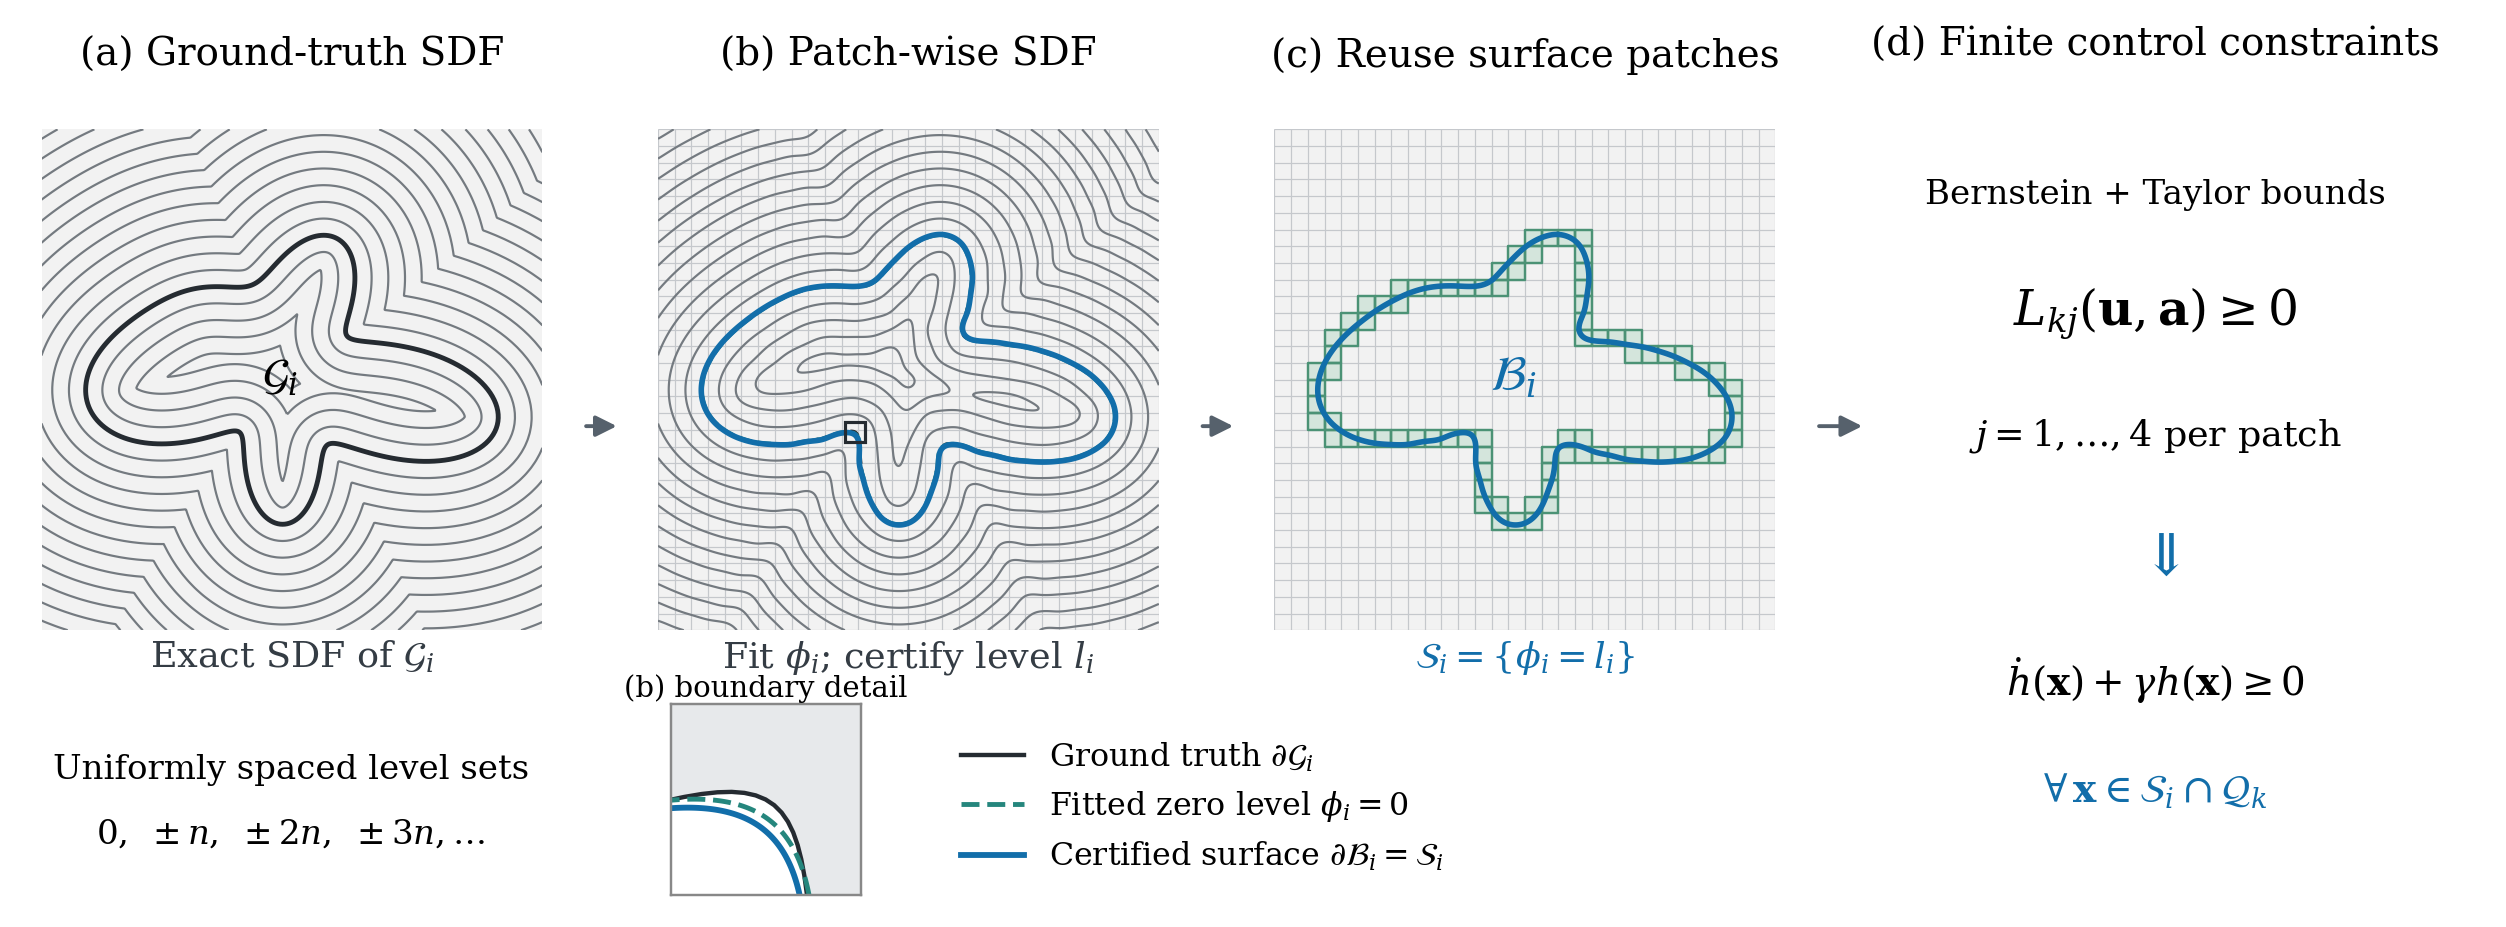
\includegraphics[width=\textwidth]{patch_pipeline.png}
\caption{From irregular geometry to finite control constraints. (a) Exact signed distance to the
ground-truth polygon $\mathcal G_i$. (b) Fitted B-spline field $\phi_i$. Both fields use the same
1.2-m-square domain and uniformly spaced, unlabeled contours (4-cm spacing).
The 4.8-cm boundary detail compares ground truth (black), the fitted zero
level (dashed teal), and the certified level set $\mathcal S_i=\{\phi_i=l_i\}$ (blue).
(c) All native patches remain visible in gray; green marks the 86 patches whose Bernstein
coefficient intervals contain $l_i=2.0$~mm. Patch size is 4~cm, without subdivision.
(d) Four affine inequalities per planar patch suffice for the CBF condition at every surface
point in that patch. $L_{kj}$ is the left side of~\eqref{eq:coef}, with its auxiliary
absolute-value bounds enforced; no surface samples define the safe set.}
\label{fig:patch-pipeline}
\end{figure*}

\begin{figure}[t]
\centering
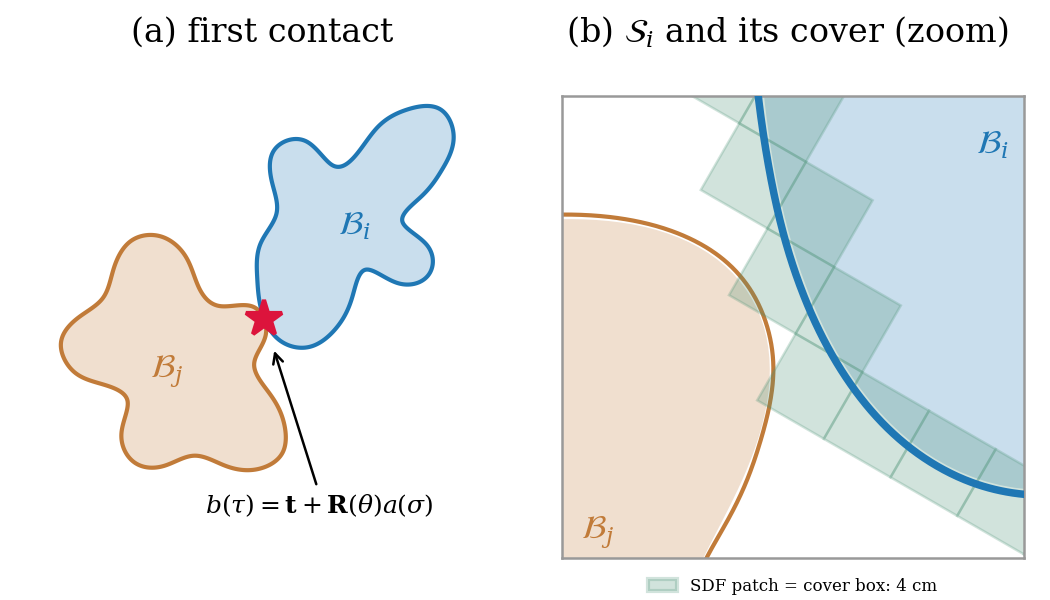
\includegraphics[width=\columnwidth]{overview.png}
\caption{The construction for two planar bodies. (a) Every first contact occurs at a
configuration $\mathbf t=b(\tau)-\Rot(\theta)a(\sigma)$ that joins boundary points of both bodies
(Lemma~\ref{lem:contact}). (b) Surface cover (Sec.~\ref{sec:cover}), with $\mathcal B_i$ 3~cm before
contact: the safe set requires $\mathcal B_j$'s SDF to stay above its certified level on
every point of the continuous certified curve $\mathcal S_i$ (thick blue); the native 4-cm SDF patches that cover
$\mathcal S_i$ (uniform green fill) only partition it to generate the
constraints on the inputs. Pale blue and amber fills show ground truth, with darker boundaries
of the same hue for the certified curves of $\mathcal B_i$ and $\mathcal B_j$, respectively.
Each retained SDF patch is one cover box, without subdivision.
The illustrated fields use 4-cm cells (690 and 650 patches for $\mathcal B_i$ and $\mathcal B_j$)
and certified levels of 2.8 and 1.9~mm.}
\label{fig:overview}
\end{figure}

\subsection{Contributions}
\begin{enumerate}
\item \emph{Boundary reduction and certified regions} (Sec.~\ref{sec:regions}): a first-contact
lemma for compact bodies in $\R^n$, and certified levels of fitted SDFs that place the true
boundaries strictly inside their sublevel regions, for polygons, triangle meshes, and exact SDFs
(resolves L3).
\item \emph{Surface-cover barriers} (Sec.~\ref{sec:cover}): a safe set defined on the continuous level
set of each body's SDF, enforced through Bernstein and vertex constraints on a lifted barrier over a
Bernstein cover of that level set, with certified Taylor remainders from third-derivative bounds;
the constraints are affine in the inputs of planar robots and in the joint velocities of
manipulators. The cover leaves the continuous safe set unchanged, while its finite certificate
restricts the admissible inputs and may affect feasibility. Arbitrary subdivision certifies every
strictly feasible input (Proposition~\ref{prop:complete}); no closest points or auxiliary geometric
optimization are needed (resolves L1 and L2).
\item \emph{Evaluation} (Sec.~\ref{sec:exp}): planar docking, multi-robot, and static-obstacle
experiments against closest-point and bounding-circle barriers, a 7-DOF Franka Panda among
non-convex obstacles against sphere, surface-sample, and closest-point barriers, and two Pandas in a
shared workspace.
\end{enumerate}

\subsection{Relation to Prior Work}\label{sec:relation}
This article keeps the problem formulation, the Bernstein-form distance fields, the pairwise
multi-robot QP, and the experimental protocol of~\cite{jo2026geometry}. It replaces the
closest-point barrier (retained as a baseline), the bounding-circle configuration space, and the
heuristic margin. New are the first-contact reduction, the certified levels, the surface-cover
barrier with its certificates and derivatives, the feasibility result, and all experiments. The
certified enclosure of planar boundaries by B-spline curves, used here for the planar baselines, and
the conversion of B-splines to Bernstein form follow~\cite{jo2027semantic} and are not claimed as
contributions.

% -----------------------------------------------------------------------------
\section{Related Work}\label{sec:related}

\emph{Geometric barriers.} Pairwise barriers between discs or spheres are the standard multi-robot
certificates~\cite{wang2017safety}, and super-ellipsoids extend them to elongated
vehicles~\cite{wang2017quadrotors}; unions of primitives multiply the constraints. For convex
polytopes, signed distances through convex programs in the Minkowski-difference space yield exact
barriers~\cite{chen2025minkowski,chen2026exact}, and smooth barriers exist between strongly convex
regions~\cite{thirugnanam2025strongly}; non-convex bodies must be decomposed. Explicit smooth
barriers for polygons compose edge-wise bounds with smooth extrema~\cite{wu2025optimization}.
Sampled distance functions yield nonsmooth barriers with quantified sampling
error~\cite{lutkus2025sampling}, and diffeomorphisms to ball worlds handle non-convex unsafe sets
without undesired equilibria~\cite{notomista2021nonconvex}.
Nonsmooth barrier compositions also handle minimum and maximum operators through differential
inclusions~\cite{glotfelter2017nonsmooth}; switching features do not invalidate that entire class.
Our closest-point baseline tests the single-minimizer derivative used in the prior formulation.

\emph{Distance fields for manipulators.} Bernstein-polynomial distance fields of articulated robots
support whole-body collision avoidance, with obstacle points queried against the robot
field~\cite{li2024representing}; neural configuration-space distance functions serve as CBFs with
robust margins~\cite{long2025neural}, and differentiable distance fields map obstacle motion into
joint space~\cite{chi2024safe}. These works establish distance fields as barriers; they do not
certify that the constraint holds on the whole continuous surface of the fitted or true geometry,
which is what our surface covers provide.

\emph{Configuration-space obstacles and Bernstein bounds.} Configuration-space obstacles of polygons
can be constructed exactly~\cite{lozanoperez1983spatial,latombe1991robot} or by grid
convolution~\cite{kavraki1995fft}, but one per pair of shapes, over all relative poses; our fields
are per body and never form them. Sum-of-squares programs can certify polyhedral collision-free
regions in a rational parametrization of configuration space~\cite{dai2024certified}.
Those region certificates and our continuous-surface input certificates address different
representations of safety. The
convex-hull property and de~Casteljau subdivision give rigorous, successively tighter bounds on
polynomials over boxes~\cite{farin2002curves,sherbrooke1993computation}; they were used
in~\cite{jo2027semantic} to certify planar spline enclosures, and we use them in up to three
variables on tensor-product fields.

% -----------------------------------------------------------------------------
\section{Preliminaries and Problem Statement}\label{sec:prelim}

\emph{CBFs.} Consider $\dot{\mathbf z}=f(\mathbf z)+g(\mathbf z)\mathbf u$ with $f,g$ locally
Lipschitz, $\mathbf u\in\mathcal U$, and a $C^1$ function $h$ with
$\mathcal H=\{\mathbf z\mid h(\mathbf z)\ge0\}$.
\begin{lemma}[\cite{ames2019cbf}]\label{lem:cbf}
If a locally Lipschitz feedback $\mathbf k(\mathbf z)\in\mathcal U$ satisfies
$L_fh+L_gh\,\mathbf k\ge-\gamma h$ with $\gamma>0$ on an open set containing $\mathcal H$, then
$\mathcal H$ is forward invariant.
\end{lemma}

\emph{Bernstein form.} The cubic Bernstein basis $B_r(\xi)=\binom3r\xi^r(1-\xi)^{3-r}$ is
nonnegative and sums to one, so $p=\sum_r\beta_rB_r$ satisfies $\min_r\beta_r\le p\le\max_r\beta_r$
on $[0,1]$ (convex-hull property), also for tensor products. With $M_B$ mapping Bernstein to power
coefficients and $T_{jr}=\binom rj\xi_0^{r-j}\Delta^j$ ($j\le r$), the coefficients of $p$ restricted
to $[\xi_0,\xi_0+\Delta]$ and reparametrized to $[0,1]$ are
\begin{equation}\label{eq:subdiv}
\boldsymbol\beta'=S(\xi_0,\xi_0+\Delta)\,\boldsymbol\beta,\qquad S=M_B^{-1}T(\xi_0,\Delta)M_B,
\end{equation}
applied along each axis; they converge to the values of $p$ as $\Delta\to0$. On each span, a uniform
cubic B-spline with control values $\mathbf P_c,\dots,\mathbf P_{c+3}$ has Bernstein coefficients
\begin{equation}\label{eq:b2b}
\boldsymbol\beta_c=Q\,[\mathbf P_{c},\dots,\mathbf P_{c+3}]^{\top},\quad
Q=\tfrac16\left[\begin{smallmatrix}1&4&1&0\\0&4&2&0\\0&2&4&0\\0&1&4&1\end{smallmatrix}\right],
\end{equation}
so bounds on a tensor-product spline, and on its derivatives, follow from finitely many
coefficients per cell~\cite{farin2002curves,jo2027semantic}.

\emph{Problem.} Robot bodies and obstacles are compact sets $\mathcal G_i\subset\R^n$, $n\in\{2,3\}$
(the \emph{ground truth}, not necessarily convex), rigidly attached to frames with poses
$(\Rot_i,\mathbf p_i)$ that depend on the state: the pose of a mobile robot, or the forward
kinematics of a link. Given nominal inputs, find minimally modified inputs under which no two
bodies ever intersect, with constraints whose correctness is certified rather than sampled.

% -----------------------------------------------------------------------------
\section{Certified Regions and First Contact}\label{sec:regions}

\subsection{First Contact}
\begin{lemma}[First contact]\label{lem:contact}
Let $\mathcal K_A(s),\mathcal K_B(s)\subset\R^n$, $s\in[0,T]$, be images of compact sets under rigid
motions that are continuous in $s$, disjoint at $s=0$ and intersecting at $s=T$. Then at
$s^\star=\inf\{s\mid\mathcal K_A(s)\cap\mathcal K_B(s)\neq\emptyset\}>0$, some point lies on both
boundaries, $\partial\mathcal K_A(s^\star)\cap\partial\mathcal K_B(s^\star)\neq\emptyset$.
\end{lemma}
\begin{proof}
The set of intersecting parameters is closed, so the bodies intersect at $s^\star>0$; pick $\mathbf z$
in both. If $\mathbf z$ were interior to $\mathcal K_B(s^\star)$, the point of $\mathcal K_A$ that
is at $\mathbf z$ at $s^\star$ would, by continuity, lie in $\mathcal K_B(s)$ for $s<s^\star$ close
to $s^\star$, a contradiction. Symmetrically, $\mathbf z$ is not interior to $\mathcal K_A(s^\star)$,
since the point of $\mathcal K_B$ at $\mathbf z$ would lie in $\mathcal K_A$ before $s^\star$.
\end{proof}
The lemma requires neither convexity nor smoothness. It reduces collision avoidance to excluding
coincident boundary points, provided that the trajectory starts collision-free.

\subsection{Certified Regions}\label{sec:cert-body}
For each body we construct a sublevel region $\mathcal B_i$ of a fitted SDF and certify
$\partial\mathcal G_i\subset\{\phi_i<l_i\}$. This boundary certificate suffices for the
first-contact argument below. It does not by itself establish $\mathcal G_i\subseteq\mathcal B_i$:
an unconstrained fitted field can have an interior positive bump. We do not assume full-solid
enclosure without an additional interior certificate.

\emph{Level sets of SDFs.} Let $\phi_i$ be a tensor-product cubic B-spline fitted to (approximate)
signed distances of $\mathcal G_i$ on a box $\Omega_i$, and let $\kappa_i(\mathbf c)$ be a certified
bound on $\norm{\nabla^2\phi_i}$ over the ball of radius $\rho\le h$ (the cell size) around $\mathbf c$: a
cubic B-spline whose control value $m$ is the maximum of the cellwise bounds from the Bernstein
coefficients of the second derivatives over cells $m-4,\dots,m+1$ per axis, which is $C^2$ and, its
weights being a partition of unity, bounds every cell adjacent to that of $\mathbf c$. The smallest level that encloses the boundary is
$\bar l_i=\max_{\partial\mathcal G_i}\phi_i$, and we certify it by branch-and-bound over pieces of the
boundary: triangles for a mesh, edges for a polygon, and, for a body given by an exact SDF, boxes of an
octree that may contain boundary points. Initial pieces are split until their radii are at most
the radius supported by the Hessian majorant, and all Taylor neighborhoods must lie inside the
field domain. For an exact SDF, a box is excluded only when
$|\mathrm{SDF}(\mathbf c)|>\rho$. For a piece $\mathcal T$ with center $\mathbf c$ and radius
$\rho$ (every point within $\rho$ of $\mathbf c$), Taylor's theorem gives
\begin{equation}\label{eq:level-ub}
\max_{\mathcal T}\phi_i\le\mathrm{UB}(\mathcal T)=\phi_i(\mathbf c)+\norm{\nabla\phi_i(\mathbf c)}\rho
+\tfrac12\kappa_i(\mathbf c)\rho^2 ,
\end{equation}
and $\phi_i$ at vertices, centers, or certified projected points on $\partial\mathcal G_i$ gives
attained values whose maximum $\ell$ lower-bounds $\bar l_i$. Mesh and polygon centers are always
included. For each retained octree box we
require a boundary point within $C\rho$ of its center and include its field value in $\ell$,
with a constant $C$ independent of refinement; for an exact SDF, a nearest boundary point gives $C=1$ when
$|\mathrm{SDF}(\mathbf c)|\le\rho$. This is a requirement on the boundary oracle, not a
consequence of evaluating a fitted field. Pieces with $\mathrm{UB}<\ell+\epsilon$ are discarded;
the others are split (a triangle into four, an edge or a box into halves or octants) and re-bounded.
\begin{proposition}\label{prop:level}
When no piece is left, $l_i=\ell+\epsilon$ satisfies $\partial\mathcal G_i\subset\{\phi_i<l_i\}$ and
$l_i\le\bar l_i+\epsilon$. With uniformly bounded derivative majorants and the boundary-point
condition above, the procedure terminates for every $\epsilon>0$.
\end{proposition}
\begin{proof}
Every boundary point lies in a discarded piece, where $\phi_i\le\mathrm{UB}<\ell+\epsilon$ with $\ell$
nondecreasing, and $\ell\le\bar l_i$ because it is attained. For mesh triangles and polygon
edges, the center is a boundary evaluation, so $\phi_i(\mathbf c)\le\ell$.
For an octree box, its boundary point $\mathbf b$ gives
$\phi_i(\mathbf c)\le\phi_i(\mathbf b)+GC\rho\le\ell+GC\rho$, where $G$ is a uniform gradient bound
on the relevant neighborhood. Hence in both cases
$\mathrm{UB}-\ell\le G(1+C)\rho+\tfrac12\kappa\rho^2$, taking $C=0$ for on-boundary centers.
Uniform subdivision makes this bound smaller than $\epsilon$ after finitely many levels.
Each level has finitely many pieces, which proves termination.
\end{proof}
The bounds certify the whole continuous boundary, with tightness up to $\epsilon$ under the
conditions above. Boundary evaluations supply lower bounds; Taylor bounds control the points
between them. The fit affects the resulting level, while the enclosure inequality follows from
the certificate, so the training targets may be approximate. We set $\mathcal B_i=\{\phi_i\le l_i\}$ and write
$\mathcal S_i=\{\phi_i=l_i\}$ for the \emph{certified surface}.

For a union of primitives, the minimum of their exact SDFs is 1-Lipschitz and exact outside
the union, but need not be the exact interior distance. It still supports conservative box
exclusion. An exterior point $\mathbf p$ with distance $d>0$ supplies the lower bound
$\phi_i(\mathbf p)-\norm{\nabla\phi_i(\mathbf p)}d-\kappa_i(\mathbf p)d^2/2$ at a true nearest
boundary point, when the majorant covers that ball. Zero values on internal seams are not
boundary evaluations. If a work limit leaves unresolved pieces, returning the larger of
$\ell+\epsilon$ and their maximum upper bound plus $\epsilon$ preserves strict boundary
inclusion; tightness to $\epsilon$ is then not claimed. The historical implicit-obstacle
levels used numerical projections and completed their upper-bound queues, establishing
the boundary enclosure but not the projection oracle required for the tightness statement.

% -----------------------------------------------------------------------------
\section{Surface-Cover Barriers}\label{sec:cover}
We keep one SDF per body and enforce the first-contact condition on the whole certified surface; the
construction is the same for planar and spatial bodies, rigid or articulated. Let body $A$ (e.g., a
robot or a link) have the certified surface $\mathcal S_A=\{\phi_A=l_A\}$ in its frame, and let body $B$
(e.g., another robot or an obstacle) have the field $\phi_B$ and level $l_B$ in its frame, both from
Proposition~\ref{prop:level}. We write $\mathbf y(\mathbf x)$ for a point $\mathbf x$ of $A$ mapped into
$B$'s frame by the current relative pose. For planar bodies, the fields are bivariate and the boxes
below are squares.

\emph{Finite domains.} We require $\phi_i>l_i$ on the boundary of each rectangular domain
$\Omega_i$, which can be certified from its boundary-cell Bernstein coefficients. For defining
the surface condition globally, extend the field by $\phi_i(\Pi_{\Omega_i}\mathbf x)$ outside
$\Omega_i$, where $\Pi_{\Omega_i}$ clips each coordinate to the domain. This extension is locally
Lipschitz, is positive above $l_i$ outside the domain, and preserves the sublevel region and its
level set. Derivatives and Taylor models are used only within the original domain.

\subsection{Safe Set on the Continuous Surface}
The safe set is the first-contact condition on every point of the certified surface,
\begin{equation}\label{eq:safe}
\mathcal H_{AB}=\big\{\text{poses}\ \big|\ h(\mathbf x)=\phi_B(\mathbf y(\mathbf x))-l_B\ge0\ \ \forall\mathbf x\in\mathcal S_A\big\};
\end{equation}
no box, sample, or bound enters its definition. We preserve this continuous spline-defined set
and construct finite Bernstein certificates for its admissible controls. Surface separation alone
does not exclude pre-existing containment of one body inside the other; collision avoidance uses
the initialization in the following theorem.
\begin{theorem}\label{thm:cover}
Suppose $\{\phi_A\le l_A\}$ and $\{\phi_B\le l_B\}$ are compact subsets of the interiors of their domains and
the strict boundary certificates of Proposition~\ref{prop:level} hold. Suppose initially
$\mathcal G_A\cap\mathcal G_B=\emptyset$ and
$\{\phi_A\le l_A\}\cap\{\phi_B<l_B\}=\emptyset$.
If a continuous trajectory stays in $\mathcal H_{AB}$, then $\mathcal G_A$ and $\mathcal G_B$
never intersect. All set intersections are understood in a common spatial frame.
\end{theorem}
\begin{proof}
For $\epsilon>0$, if $\{\phi_A\le l_A\}$ met $\{\phi_B\le l_B-\epsilon\}$, Lemma~\ref{lem:contact} would
give a first point on both boundaries, where $\phi_A=l_A$ and $\phi_B=l_B-\epsilon$, contradicting
$h\ge0$ on $\mathcal S_A$. Hence $\{\phi_A\le l_A\}\cap\{\phi_B<l_B\}=\emptyset$ throughout. A first
contact of $\mathcal G_A$ and $\mathcal G_B$ would lie on $\partial\mathcal G_A\cap\partial\mathcal G_B$
(Lemma~\ref{lem:contact}), where $\phi_A<l_A$ and $\phi_B<l_B$ by Proposition~\ref{prop:level}.
\end{proof}

\subsection{Certified Cover and Lifted Barrier}
On each cell of $\phi_A$, the Bernstein coefficients of $\phi_A-l_A$ follow from~\eqref{eq:b2b}. If
they all have one strict sign on a box, the box contains no point of $\mathcal S_A$ by the
convex-hull property. The converse need not hold: a retained box may contain no surface point.
The default retains each native SDF cell whose coefficient interval contains zero, without
subdividing it. These patches are the boxes $\{\mathcal Q_k\}$, with side $s=h_A$ fixed by the SDF
grid, centers $\mathbf c_k$, and half-diagonal $r=\sqrt n\,s/2$; their union contains all of
$\mathcal S_A$. There is no independent cover-size parameter. Optionally, retained patches can be
halved using~\eqref{eq:subdiv}, discarding children whose coefficient intervals exclude zero.
The cover is computed once per body; it only partitions
the surface for the enforcement below and does not enter~\eqref{eq:safe}. Subdivision restricts the
same polynomial to smaller domains; it neither samples nor refits the surface.

By the comparison lemma, $\mathcal H_{AB}$ stays invariant if $\dot h(\mathbf x)\ge-\gamma h(\mathbf x)$
at every surface point. The surface is implicit, so we impose this condition on whole boxes, after
lifting the barrier to reduce the tightening caused by points off the surface: for $\mathbf x$ in a
box,
\begin{equation}\label{eq:lift}
\tilde h(\mathbf x)=\phi_A(\mathbf x)-l_A+\phi_B(\mathbf y(\mathbf x))-l_B ,
\end{equation}
which equals $h$ on $\mathcal S_A$. Since $\mathbf x$ is fixed in $A$'s frame, $\phi_A(\mathbf x)$ does
not change, and $\dot{\tilde h}(\mathbf x)=\nabla\phi_B(\mathbf y)^\top\dot{\mathbf y}(\mathbf x)$. A
box point displaced from the surface by $\delta$ toward $B$ has $\phi_A-l_A\approx\delta$ and
$\phi_B-l_B\approx h-\delta$ for SDF-like fields, so $\tilde h\approx h$: the lifting cancels the
first-order effect only to the extent that the opposing gradients cancel. The box points move with
$\dot{\mathbf y}(\mathbf x)=\mathbf J\mathbf u+\mathbf W(\mathbf u)(\mathbf y-\mathbf y_{\mathbf c})$,
affine in the inputs $\mathbf u$, where $\mathbf J\mathbf u$ is the velocity of the box center in
$B$'s frame and $\mathbf W(\mathbf u)$ the relative angular velocity as a skew matrix
(Sec.~\ref{sec:cover-der}).

\subsection{Bernstein and Vertex Constraints}
A box in $A$'s frame can cross several knot cells of $B$ after a rigid transformation.
Certified Taylor models avoid constructing their intersections online. These models are used
only to bound the control inequality; the represented surfaces and certified levels remain
those of the original splines.
Cellwise bounds on the Frobenius norm of the third-derivative tensor follow from the Bernstein
coefficients of the third partial derivatives. A tensor-product cubic B-spline is $C^2$ with bounded,
piecewise-polynomial third
derivatives, so its Hessian is Lipschitz with these bounds on any region they cover, which is what the
third-order Taylor remainders below require. On each (fixed) box of $A$, $M_A$ is their maximum over
all cells meeting the bounding cube of half-width $r$ around its center, including for a full
native patch. For $\phi_B$, the bound must vary continuously with the pose:
$M_B$ is piecewise multilinear on a grid of spacing $h/2$, with node values the maxima over the cells meeting
the cube of half-width $h/2+r$ around the node; interpolation is a convex combination of nodes whose
cubes all contain the ball of radius $r$ around $\mathbf y_{\mathbf c}$, so $M_B$ bounds the tensor on
that ball and is Lipschitz. Let $q_A$ and $q_B$ be the second-order Taylor polynomials of
$\phi_A$ at $\mathbf c$ and of $\phi_B$ at $\mathbf y_{\mathbf c}$. Taylor's theorem gives, on a box,
$\phi_A\ge q_A-\tfrac16M_Ar^3$, $\phi_B\ge q_B-\tfrac16M_Br^3$, and
$\norm{\nabla\phi_B-\nabla q_B}\le\tfrac12M_Br^2$. The box points move relative to $B$ with the twist
$(\mathbf V,\boldsymbol\Omega)$ of $A$ relative to $B$ at $A$'s origin $\mathbf p_A$, linear in $\mathbf u$,
so $\norm{\dot{\mathbf y}(\mathbf x)}\le\norm{\mathbf V}_1+\rho\norm{\boldsymbol\Omega}_1$ with
$\rho=\norm{\mathbf c}+r$, since $\mathbf c$ is expressed in $A$'s body frame.
With $\mathbf d=\mathbf y-\mathbf y_{\mathbf c}$, $\norm{\mathbf d}\le r$,
$\mathbf g=\nabla\phi_B(\mathbf y_{\mathbf c})$, $\mathbf H=\nabla^2\phi_B(\mathbf y_{\mathbf c})$, and
$\dot{\mathbf y}_{\mathbf c}=\mathbf J\mathbf u$, the models give on the box
\begin{equation}\label{eq:psi-lb}
\begin{aligned}
\Psi\ge{}&\mathbf g^\top\dot{\mathbf y}_{\mathbf c}+\mathbf d^\top\mathbf H\dot{\mathbf y}_{\mathbf c}
+\mathbf g^\top\mathbf W\mathbf d-r^2\norm{\mathbf H}\norm{\boldsymbol\Omega}\\
&+\gamma\big(q_A-l_A+q_B-l_B-\tfrac16(M_A+M_B)r^3\big)\\
&-\tfrac12M_Br^2\big(\norm{\mathbf V}_1+\rho\norm{\boldsymbol\Omega}_1\big),
\end{aligned}
\end{equation}
where $\Psi(\mathbf x,\mathbf u)=\nabla\phi_B(\mathbf y)^\top\dot{\mathbf y}(\mathbf x)+\gamma\tilde h(\mathbf x)$;
the first three terms are affine in $\mathbf d$ and in $\mathbf u$.

\emph{Joint coefficient certificate.} Before bounding the terms separately as
in~\eqref{eq:psi-lb}, one can retain the full quadratic model. More generally, write
$g_A=\phi_A-l_A$ and $F=\dot h+\gamma h$. For any scalar $w$ held constant over a box,
$F+\gamma w g_A=F$ on $\mathcal S_A$. Define
\begin{equation}\label{eq:joint-model}
\begin{aligned}
p_w={}&(\mathbf g+\mathbf H\mathbf d)^\top
              (\mathbf J\mathbf u+\mathbf W(\mathbf u)\mathbf d)\\
 &+\gamma\big(w(q_A-l_A)+q_B-l_B\big),\\
E_w={}&\tfrac\gamma6(|w|M_A+M_B)r^3\\
 &+\tfrac12M_Br^2(\mathbf1^\top\mathbf a_V+
                       \rho\mathbf1^\top\mathbf a_\Omega).
\end{aligned}
\end{equation}
The two-sided Taylor bounds give $F+\gamma w g_A\ge p_w-E_w$.
Consequently, if $b_k(p_w)$ are its $3^n$ tensor Bernstein coefficients,
\begin{equation}\label{eq:joint-coef}
b_k(p_w)\ge E_w\quad\text{for every }k,\qquad
\mathbf a\ge|(\mathbf V,\boldsymbol\Omega)|,
\end{equation}
then the CBF condition holds on $\mathcal S_A\cap\mathcal Q$. This certificate keeps
the value and velocity terms in the same polynomial, preserving their cancellation.
For fixed $w$, its constraints are affine in $(\mathbf u,\mathbf a)$.
The unit choice $w=1$ recovers the summed-field residual. Other choices are equality
multipliers for the surface condition, not new barriers to be differentiated;
they change neither the surface nor~\eqref{eq:safe}.

\emph{Vertex reduction.} The implementation used in the main experiments reduces
the number of rows by bounding the value and velocity terms separately:
\begin{proposition}\label{prop:coef}
Let $\beta_k$, $k=1,\dots,3^n$, be the Bernstein coefficients of degree two per coordinate of
$q_A-l_A+q_B(\mathbf y(\cdot))-l_B$ on a box $\mathcal Q$, let $\mathbf d_j$, $j=1,\dots,2^n$, be the
vertices of $\mathcal Q$ relative to its center in $B$'s frame, and let
$\sigma_V=\frac12M_Br^2$ and $\sigma_\Omega=\frac12\rho M_Br^2+r^2\norm{\mathbf H}$. If, for all $j$,
\begin{equation}\label{eq:coef}
\begin{aligned}
&(\mathbf g+\mathbf H\mathbf d_j)^\top\mathbf J\mathbf u+\mathbf g^\top\mathbf W(\mathbf u)\mathbf d_j
-\sigma_V\mathbf 1^{\!\top}\mathbf a_V-\sigma_\Omega\mathbf 1^{\!\top}\mathbf a_\Omega\\
&\quad+\gamma\big(\min_k\beta_k-\tfrac16(M_A+M_B)r^3\big)\ge0,\\
&\mathbf a=(\mathbf a_V,\mathbf a_\Omega)\ge|(\mathbf V,\boldsymbol\Omega)|,
\end{aligned}
\end{equation}
then $\Psi(\mathbf x,\mathbf u)\ge0$ for every $\mathbf x\in\mathcal Q$.
\end{proposition}
\begin{proof}
In~\eqref{eq:psi-lb}, the terms affine in $\mathbf d$ attain their minimum over the (rotated) box at a
vertex, and the value model is at least $\min_k\beta_k$ by the convex-hull property; the twist terms
are bounded by $\mathbf a$.
\end{proof}
The constraints, $2^n$ per box, are affine in $(\mathbf u,\mathbf a)$. The epigraph variables $\mathbf a$ (six per pair of
bodies in space, three in the plane) are shared by all boxes of the pair, and since the left side
of~\eqref{eq:coef} decreases in $\mathbf a$, the feasible set in $\mathbf u$ is exactly that of the same
constraints with $|(\mathbf V,\boldsymbol\Omega)|$; the filter remains a QP. Joint-by-joint speed bounds
would be looser, since joint velocities partly cancel in the twist.
The remainder terms tighten only the admissible inputs, and the one
proportional to the twist vanishes at rest. Online, $\phi_B$, its first two derivatives, and $M_B$ are
evaluated at box centers; the Taylor data of $\phi_A$ are computed offline. At rest, the loss of the
constraints is bounded as follows:
\begin{proposition}\label{prop:tight}
With $\mathbf b=\nabla\phi_A(\mathbf c)+\Rot^\top\nabla\phi_B(\mathbf y_{\mathbf c})$ and
$\mathbf Q=\nabla^2\phi_A(\mathbf c)+\Rot^\top\nabla^2\phi_B(\mathbf y_{\mathbf c})\Rot$, where
$\Rot$ maps $A$'s frame to $B$'s, the constant terms of~\eqref{eq:coef} are at least
$\gamma\big(\tilde h(\mathbf c)-\tfrac s2\norm{\mathbf b}_1-\tfrac{s^2}8\sum_{ij}|Q_{ij}|
-\tfrac16(M_A+M_B)r^3\big)$.
\end{proposition}
\begin{proof}
With $\mathbf x=\mathbf c+s\boldsymbol\tau$, $\boldsymbol\tau\in[-\frac12,\frac12]^n$, the degree-two
coefficients of $\tau_i$, $\tau_i\tau_j$, and $\tau_i^2$ lie in $[-\frac12,\frac12]$,
$[-\frac14,\frac14]$, and $[-\frac14,\frac14]$.
\end{proof}
The first-order term vanishes only where the two gradients cancel, $\nabla\phi_A=-\Rot^\top\nabla\phi_B$:
exact SDFs satisfy this at a smooth external tangency where both gradients exist; fitted fields
need not satisfy it, since
their gradients may differ in norm and in direction. A first-order ball bound on $\phi_B$ alone
subtracts $\norm{\nabla\phi_B}r$ even there. The proposition concerns the constant terms at rest; the velocity
terms of~\eqref{eq:coef} add their own, input-dependent loss.

\subsection{Derivatives and Pruning}\label{sec:cover-der}
For planar $SE(2)$ single integrators, a point of $A$ at world position $\mathbf w$ moves in $B$'s frame
with $\Rot(\theta_B)^{\!\top}\big(\mathbf v_A+\omega_AJ(\mathbf w-\mathbf p_A)-\mathbf v_B-\omega_BJ(\mathbf w-\mathbf p_B)\big)$,
$J=\left[\begin{smallmatrix}0&-1\\1&0\end{smallmatrix}\right]$, and
$\mathbf W=(\omega_A-\omega_B)J$. For a link $A$ of an articulated robot, a revolute joint $j$ before
the link contributes the column $\mathbf z_j\times(\mathbf w-\mathbf o_j)$ and the angular velocity
$\mathbf z_j\dot q_j$; for two moving arms, the joints of $B$'s arm enter with the opposite sign. In
every case, $\mathbf J$ and $\mathbf W$ are linear in the inputs and are obtained directly from
the kinematics, without a closest-point optimization.
For two spatial bodies, using world-frame velocities at their origins,
$\mathbf V=\mathbf v_A-\mathbf v_B-\boldsymbol\omega_B\times(\mathbf p_A-\mathbf p_B)$ and
$\boldsymbol\Omega=\boldsymbol\omega_A-\boldsymbol\omega_B$ give
$\dot{\mathbf y}=\Rot_B^\top[\mathbf V+\boldsymbol\Omega\times(\mathbf w-\mathbf p_A)]$.
Thus $\mathbf W=[\Rot_B^\top\boldsymbol\Omega]_\times$, where $[\mathbf v]_\times\mathbf d=\mathbf v\times\mathbf d$.
The Euclidean speed bound is rotation invariant; the componentwise absolute-value bounds
use these world-frame twist coordinates throughout.

\emph{Pruning.} A box needs no constraint if the constant terms of~\eqref{eq:coef}, divided by
$\gamma$, are at least an activation threshold $\eta>0$: then $h\ge\eta$ on its part of the surface.
We group the boxes of each body into clusters with center $\bar{\mathbf c}$ and radius $R$ (covering
the boxes' balls) and skip a cluster if $\phi_B(\mathbf y(\bar{\mathbf c}))-GR-l_B+\min(\phi_A-l_A)\ge\eta$,
where $G$ bounds $\norm{\nabla\phi_B}$ on the cells the cluster can reach and the minimum of
$\phi_A-l_A$ over the cluster's boxes is certified offline; remaining boxes are first screened with
$\phi_B(\mathbf y_{\mathbf c})-\norm{\nabla\phi_B(\mathbf y_{\mathbf c})}r-\frac12\kappa_B(\mathbf y_{\mathbf c})r^2-l_B+\min_{\mathcal Q}(\phi_A-l_A)\ge\eta$.
If $r>h_B$, the Hessian majorant uses the same radius-dependent window construction as $M_B$.

\emph{Domain-boundary pruning.} A box whose enclosing ball is not contained in $\Omega_B$
cannot use that Taylor model. If $r_{\max}$ bounds the half-diagonal of every cover box paired
with $B$, certify offline that $\phi_B-l_B\ge\delta_B>0$ on the inner domain collar of width
$2r_{\max}$. Bernstein coefficients of all cells meeting the collar give such a bound.
Every point of a box omitted by the radius-$r$ containment test either lies in this collar or
outside the domain, where the clipped extension has the same positive bound. Thus $h\ge\delta_B$
on its surface portion. The comparison proof uses the effective threshold
$\eta_0=\min(\eta,\delta_B)$; the implementation may still activate in-domain boxes at the larger
$\eta$. Domain padding alone is not a certificate: if the collar bound fails, the box needs an
alternative certified treatment. Clusters that leave the domain are checked box by box.

\emph{Optional refinement.} The default uses native patches and performs no online refinement.
Where the field varies rapidly, $\frac12M_Br^2$ can exceed
$\norm{\nabla\phi_B}$: the bound then fails to resolve the gradient direction and can reject useful
motion, causing a stall. An active box
with $\frac12M_Br^2>\vartheta$ is therefore replaced online by those of its $2^n$ half-size boxes whose
bounds of $\phi_A-l_A$ bracket zero; they cover the same part of $\mathcal S_A$.
For unchanged derivative bounds, halving $r$ quarters the gradient remainder and reduces the
value remainder by a factor of eight. The subdivided implementation uses $\vartheta=0.1$ and at most two halvings.
The original experiments additionally limit refinement to boxes whose lower bound of $\tilde h$
is below 1~cm, except for the tube scene; the common distance-independent rule is evaluated
in the certificate comparison below.
\begin{theorem}\label{thm:invariance}
Consider an absolutely continuous pose trajectory with measurable inputs satisfying the
kinematic dynamics almost everywhere, initially in $\mathcal H_{AB}$. Suppose that for almost
every time, each cover box (or its retained refined children) either has a certificate
$h\ge\eta_0>0$ on its surface portion, or satisfies~\eqref{eq:coef} or~\eqref{eq:joint-coef}
with the applied input and valid auxiliary bounds. Then the trajectory remains in $\mathcal H_{AB}$.
\end{theorem}
\begin{proof}
Fix $\mathbf x\in\mathcal S_A$ and write $h_{\mathbf x}(t)=h(\mathbf x,t)$, which is absolutely
continuous. Where $h_{\mathbf x}<\eta_0$, no box containing $\mathbf x$ can be excluded by a
positive surface bound. The finite certificate and the chain rule therefore give
$\dot h_{\mathbf x}\ge-\gamma h_{\mathbf x}$ almost everywhere there. If $h_{\mathbf x}(t_1)<0$,
continuity gives a last zero $t_0<t_1$, with $h_{\mathbf x}<0$ on $(t_0,t_1]$.
The absolutely continuous function $e^{\gamma t}h_{\mathbf x}(t)$ has nonnegative derivative
almost everywhere on that interval, contradicting $h_{\mathbf x}(t_1)<0$. This argument applies
separately to every fixed surface point; no common exceptional time set over all points is needed.
\end{proof}

\begin{proposition}[Certification of strictly feasible inputs]\label{prop:complete}
Fix a pose and input $\mathbf u$. Suppose $\mathcal S_A$ is compact, its mapped neighborhood lies
inside the field domains, and $F(\mathbf x,\mathbf u)\ge\epsilon>0$ on $\mathcal S_A$.
Assume uniformly bounded derivative majorants on that neighborhood. If subdivision is allowed
to arbitrary depth, with consistent exclusion bounds for $g_A$, then a finite subdivision
certifies this input using either~\eqref{eq:coef} or~\eqref{eq:joint-coef} with $w=1$.
\end{proposition}
\begin{proof}
The unit lifted residual equals $F$ on the surface. Continuity and compactness give a neighborhood
where it is at least $\epsilon/2$. As the maximum box diameter tends to zero, consistent exclusion
bounds discard boxes bounded away from the surface. The remaining boxes eventually lie in that
neighborhood. Bernstein enclosure errors, the losses from separating the terms, and the Taylor
remainders converge uniformly to zero for the fixed input. Eventually their sum is smaller than
$\epsilon/2$, so every retained box passes its certificate.
\end{proof}
This result concerns optional subdivision and strictly feasible inputs, not completeness of the
fixed native-patch certificate or finite certification of inputs with $F=0$.
The two-level subdivided implementation has a finite computational budget. Re-centering Taylor models can
also prevent successive finite certificates from being nested.

% -----------------------------------------------------------------------------
\section{Safety Filter}\label{sec:filter}
Collecting the constraints~\eqref{eq:coef} of the active boxes of all pairs, the filter is
\begin{equation}\label{eq:qp}
\begin{aligned}
(\mathbf u^\ast,\mathbf a^\ast)=\argmin_{\mathbf u\in\mathcal U,\,\mathbf a}\ &\norm{\mathbf u-\mathbf u^{\rm nom}}^2+\varepsilon_a\norm{\mathbf a}^2\\
\text{s.t. }&\eqref{eq:coef}\ \text{for all active boxes},
\end{aligned}
\end{equation}
with $\mathbf u$ the stacked planar velocities or the joint velocities, $\mathbf a$ the epigraph
variables of all active pairs, and $\varepsilon_a=10^{-3}$. With
polytopic input bounds, \eqref{eq:qp} is a QP, which we reformulate as a least-distance program and solve numerically by
non-negative least squares~\cite{lawson1995solving}, warm-started by constraint generation.
\begin{proposition}[Feasibility]\label{prop:feas}
For driftless dynamics---planar single integrators, unicycles, or velocity-controlled joints---and
any $\mathcal U\ni\mathbf 0$, $(\mathbf u,\mathbf a)=\mathbf 0$ is feasible for~\eqref{eq:qp} whenever
the constant terms of~\eqref{eq:coef} are nonnegative on all active boxes; by
Proposition~\ref{prop:tight}, this holds wherever $\tilde h$ at the box centers exceeds the bound given
there, which shrinks with the box size.
\end{proposition}
\begin{proof}
All velocity terms of~\eqref{eq:coef} are linear in $\mathbf u$ without drift, so
$(\mathbf u,\mathbf a)=\mathbf 0$ leaves the constant terms.
\end{proof}
\begin{corollary}\label{cor:closed}
Suppose each pair satisfies the initial conditions of Theorem~\ref{thm:cover}. If an absolutely
continuous closed-loop trajectory exists along which~\eqref{eq:qp} stays feasible and its applied
inputs satisfy the conditions of Theorem~\ref{thm:invariance} almost everywhere, then along that trajectory
no pair of ground-truth shapes intersects. The certified sublevel regions may touch at their
level boundaries.
\end{corollary}
\begin{proof}
Theorem~\ref{thm:invariance} keeps each pose in $\mathcal H_{AB}$, and Theorem~\ref{thm:cover}
concludes.
\end{proof}
Stopping is certified when the constant terms are nonnegative. A finite certificate may fail to
certify stopping near the boundary even though zero input preserves the exact safe set for the
driftless model. Proposition~\ref{prop:tight} bounds the constant-term loss; it does not give a
general physical width of this region without additional assumptions on the fields.
No step needed slack in the reported subdivided experiments, and the safe set itself is unaffected.
Feasibility does not imply progress: exact non-convex geometry can hook and block
bodies~\cite{reis2020undesirable}, and we do not resolve such deadlocks. In the experiments, a slack
variable is added only if~\eqref{eq:qp} is infeasible.

% -----------------------------------------------------------------------------
\section{Experiments}\label{sec:exp}

The default certificate uses native SDF patches with $s=h_A$ and no online refinement.
Section~\ref{sec:native} evaluates this setting with unchanged fields and levels.
The remaining experiments report the separately identified, subdivided implementation; their
clearances, success rates, and timings are not attributed to the native-patch default.
Spatial and crowded planar runs include filter times above the 10-ms simulation step;
the reported timing distributions do not establish a hard 100-Hz real-time guarantee.

\subsection{Planar Setup}
Unless stated otherwise, control uses $SE(2)$ single integrators with $\gamma=5$,
$v_{\max}=1$~m/s, $\omega_{\max}=2$~rad/s,
a 10-ms step, and a proportional nominal controller. In the subdivided planar experiments,
unless stated otherwise, each body's field is a
bivariate cubic B-spline with 1-cm cells fitted to approximate signed distances of its ground-truth polygon,
its tightest level is certified on the polygon by Proposition~\ref{prop:level} ($\epsilon=0.1$~mm),
its certified curve is covered by 5-mm boxes with four constraints~\eqref{eq:coef} each, and
$\eta=5$~cm. Computations run in Python on one thread of an AMD Ryzen~9 3900X CPU. Ground-truth
shapes are dense polygons; collisions are checked at every step and, between steps, along the
interpolated poses with a rigid-motion bound and bisection down to 0.1~mm.
Reported minima are evaluated polygon distances, not exact continuous-time minima.

\emph{Baselines.} Both baselines use certified B-spline boundaries of the bodies~\cite{jo2027semantic}
(boundary curves whose control hulls miss the ground truth after subdivision). The \emph{closest-point}
barrier is the signed distance between these fitted bodies, sampled as polygons (on an NVIDIA RTX~4070
GPU), minus a margin $m=2$~cm, with the derivative at one closest pair; it uses certified boundary
fits but keeps the single-closest-point structure of~\cite{jo2026geometry}. The \emph{circle}
barrier~\cite{wang2017safety} uses the minimum enclosing circle of each fitted body, with body-frame
center, and the same margin.

\subsection{Native-Patch Default}\label{sec:native}
We retain native patches with $s=h_A$ and disable online refinement, keeping the fields,
certified levels, nominal controllers, and initial conditions unchanged. These measurements use
one CPU thread per process; the Franka trials run in concurrent batches, with other background
activity not excluded. The timings are separate from the isolated timings
of the subdivided implementation.

In the docking scene of Sec.~\ref{sec:exp-dock}, the vehicle's 10-mm SDF patches give 772 cover
boxes. Over the same 9-s horizon, the nose seats to a depth of 0.691~m, with a minimum polygon gap
of 9.1~mm and no slack. At most 192 boxes contribute 768 constraints; median/p95 filter time is
3.08/3.67~ms. The subdivided 5-mm version seats to 0.698~m with a 1.7-mm gap
(Table~\ref{tab:dock-base}). Thus the native-patch default docks with fewer constraints but leaves
more clearance in this scene.

A separate two-robot crossing uses the fields of Fig.~\ref{fig:overview}, with 4-cm cells,
and compares 87 native cover patches against 718 boxes of 5~mm, both without online refinement.
Over 12~s, both runs avoid collision and use no slack, but neither reaches both goals.
Minimum saved-state polygon gaps are 21.4 and 4.5~mm; maximum constraint counts are 32 and 628,
and median filter times are 1.81 and 3.31~ms, respectively. A rigid-motion audit also verifies
positive gaps along the interpolated steps. This single scene illustrates the tradeoff;
subdivision does not resolve its deadlock.

On the same 30 Franka trials of Sec.~\ref{sec:exp-franka}, native 12-mm patches give 6847 boxes,
against 26{,}636 initial boxes in the subdivided implementation. Only 6 trials reach the goal
within 10~s, against 17 with subdivision. Two trials require slack (1497 steps in total), so the
hard CBF conditions are not maintained in those runs. Nevertheless, the saved-state mesh-distance
lower bounds, including final states, remain positive: the minimum is 15.3~mm and the median of
trial minima is 26.5~mm. These audits do not certify between-step motion. At most 258 boxes produce
2064 constraints; pooled median/p95 filter time is 10.5/16.7~ms under the non-isolated conditions
above. Thus removing the cover-size and refinement choices substantially reduces row counts, but
can sacrifice progress and feasibility of the finite certificate at this field resolution.

\emph{Finer native SDF patches.} To distinguish coarse field resolution from the use of native
patches, we refit all eight link fields with 6-mm cells and use those cells directly as the cover,
without subdivision or online refinement. We select the first trial in the saved ordering that
reached with the historical subdivided method but stalled with 12-mm native patches (trial index 2,
zero-based). The obstacle fields and controller are unchanged. The refitted fields have levels of
0.95--1.66~mm and 26{,}182 cover patches; the arm reaches in 5.13~s with zero slack, at most 191 active
patches (1528 constraints), and a saved-state mesh-distance lower bound of 29.7~mm. Median/p95 filter
time is 5.88/17.17~ms, including kinematics, constraint assembly, and the QP; 26.9\% of steps exceed
10~ms, so this run does not establish a 100-Hz real-time guarantee. Background activity was not
excluded. This selected trial demonstrates that finer native patches can restore progress without
a separate cover resolution; it is not a 30-trial success estimate, and refitting also changes the
fields and certified levels.

\subsection{Docking into a Tapered Receptacle}\label{sec:exp-dock}
A fixed module carries two panel arrays and, in its front face, a tapered receptacle; a vehicle
has a hull, two nozzles, two panel arrays, and a 0.70-m nose that narrows from 0.32 to 0.10~m
(Fig.~\ref{fig:dock}). The receptacle is the seated nose offset outward by 32~mm everywhere, so the
nose seats fully (0.668~m past the mouth) only if the barrier admits configurations within 32~mm of
contact, and only within a narrow band of orientations. The module and vehicle fields have 1.25- and
1-cm cells, their tightest levels certified on the ground-truth polygons are 1.2 and 0.5~mm, and 1548
boxes of 5~mm cover the vehicle's certified curve; the baselines' certified boundaries need offsets
of 4 and 5~mm. The vehicle starts 3.4~m away, rotated by $40^\circ$, and its nominal goal lies 10~cm
past full seating.

\begin{figure*}[t]
\centering
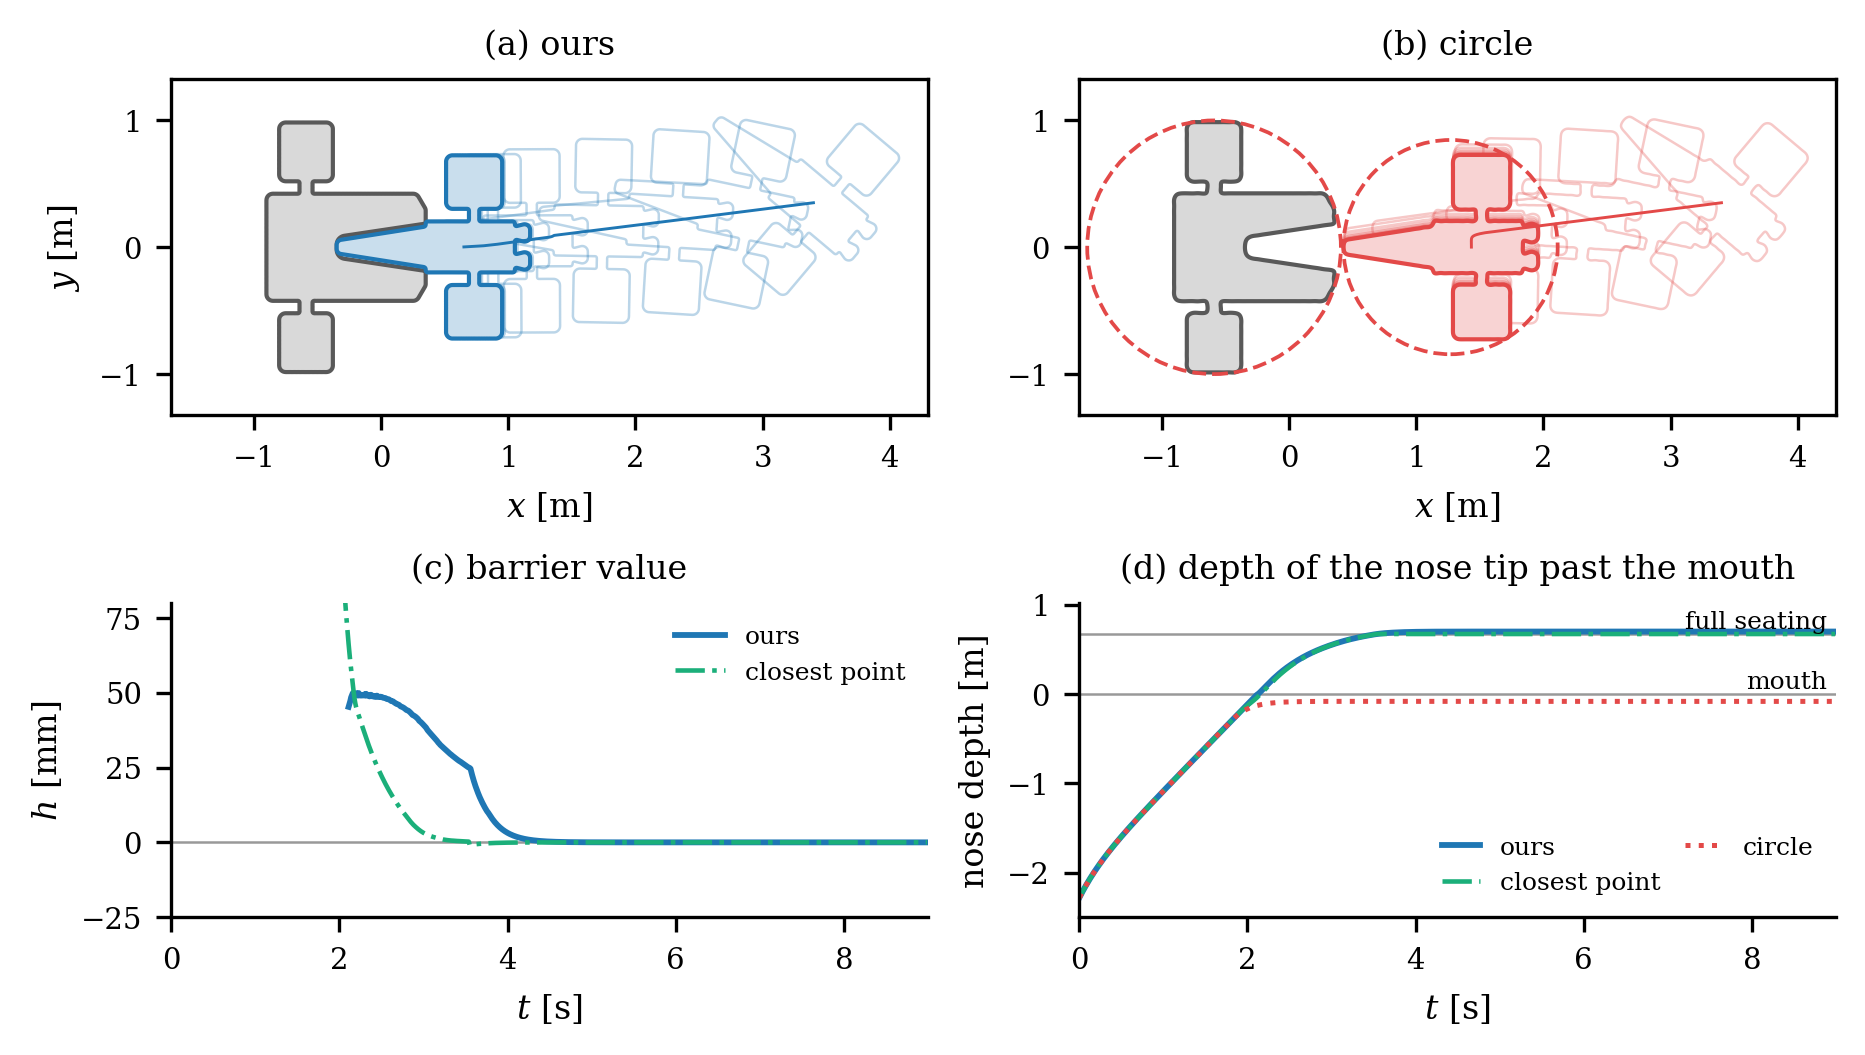
\includegraphics[width=\textwidth]{dock_paper.png}
\caption{Docking into a tapered receptacle with the module fixed. (a) Surface-cover barriers: the
vehicle rotates while approaching and seats its 0.70-m nose 3.0~cm past full seating, 1.7~mm from the
receptacle floor. (b) Minimum enclosing circles (dashed): the vehicle stops 8~cm in front of the
mouth. Poses every 0.6~s; pale fills: ground truth; darker outlines of the same hue: certified
boundaries. The fixed module uses light-gray fill and a dark-gray outline. (c) Barrier
value (for the cover, the certified lower bound of $\tilde h$ over the active boxes): the cover keeps
$h\ge0$, the closest-point barrier violates its constraint by 0.9~mm. (d) Depth of the nose tip past the mouth
(full seating: 0.668~m).}
\label{fig:dock}
\end{figure*}

\begin{table}[t]
\caption{Docking with Different Barriers}
\label{tab:dock-base}
\centering
\footnotesize
\setlength{\tabcolsep}{4pt}
\renewcommand{\arraystretch}{1.05}
\begin{tabular}{lccc}
\toprule
& ours & closest point & circle\\
\midrule
certified level [mm] & 1.2, 0.5 & -- & --\\
nose depth [m] & \textbf{0.698} & 0.671 & $-0.084$\\
min.\ evaluated gap [mm] & 1.7 & 28.4 & 102.5\\
min.\ $h$ [mm] & \textbf{0.0} & $-0.9$ & --\\
input variation & 6.4 & 3.8 & 2.5\\
constraints, max. & 1604 & 1 & 1\\
time per step [ms] & 6.2 & 6.5 & 0.22\\
\bottomrule
\end{tabular}
\\[3pt]
\parbox{\columnwidth}{\footnotesize Nose depth: tip past the mouth at the end (full seating with a
32-mm gap: 0.668~m). Ours: levels of the module and vehicle fields, 1548 boxes of 5~mm, at most 401
active; $h$: certified lower bound of $\tilde h$. Input variation:
$\sum_k\norm{\mathbf u_{k+1}-\mathbf u_k}_1$ in the stated SI coordinates.
Time: median, complete filter, one CPU thread. The
circle barrier's $h$ is in m$^2$ and stayed nonnegative.}
\end{table}

With the surface cover, the vehicle docks without violating its barrier and without slack
(Fig.~\ref{fig:dock}a, Table~\ref{tab:dock-base}): it rotates while approaching, and its nose passes
the full-seating depth by 3.0~cm, closing the 32-mm floor gap to 1.7~mm, close to the sum of the
two certified levels (1.2 and 0.5~mm) in this scene. Halving the 5-mm boxes to 2.5~mm changes
the gap by 0.1~mm. Barriers at the box corners that bound $\phi_B$ alone, whose safe set
depends on the boxes, stop the nose at 6.8~mm (3.9~mm with 2.5-mm boxes). The price is up to 401 active boxes with 1604 constraints.

The closest-point barrier also docks smoothly here, because the contact stays on the tapered walls and
the closest pair does not jump, but its 2-cm margin leaves 28.4~mm to the floor, and it still
violates its constraint by 0.9~mm; the circles stop the nose 8~cm in front of the mouth.

\subsection{Multiple Robots}\label{sec:exp-five}
Five shapes are generated as star-shaped radial Fourier series with hull-area ratios below 0.9,
and scaled to radii of 0.85--1.08~m. Each body needs one field: the five tightest levels
(0.29--0.35~mm) and covers (1240--1426 boxes), with the Taylor data of the boxes, take 50~s in total,
an offline cost linear in the number of bodies. The robots move to the
antipodal positions on a circle of radius 4~m under $SE(2)$ single-integrator dynamics, with start
and goal angles perturbed by up to $9^\circ$ and $20^\circ$ to avoid the central deadlock of exactly
antipodal goals. All robots reach their goals after 12.5~s (Fig.~\ref{fig:five}); the minimum
ground-truth distance is 0.8~mm, and the certified lower bound of the lifted barriers stays above
$+0.17$~mm. While all five crowd the center, up to 2716 constraints are active, and the cost per step
rises from 2.8~ms (median) to 22~ms (95th percentile).

\begin{figure}[t]
\centering
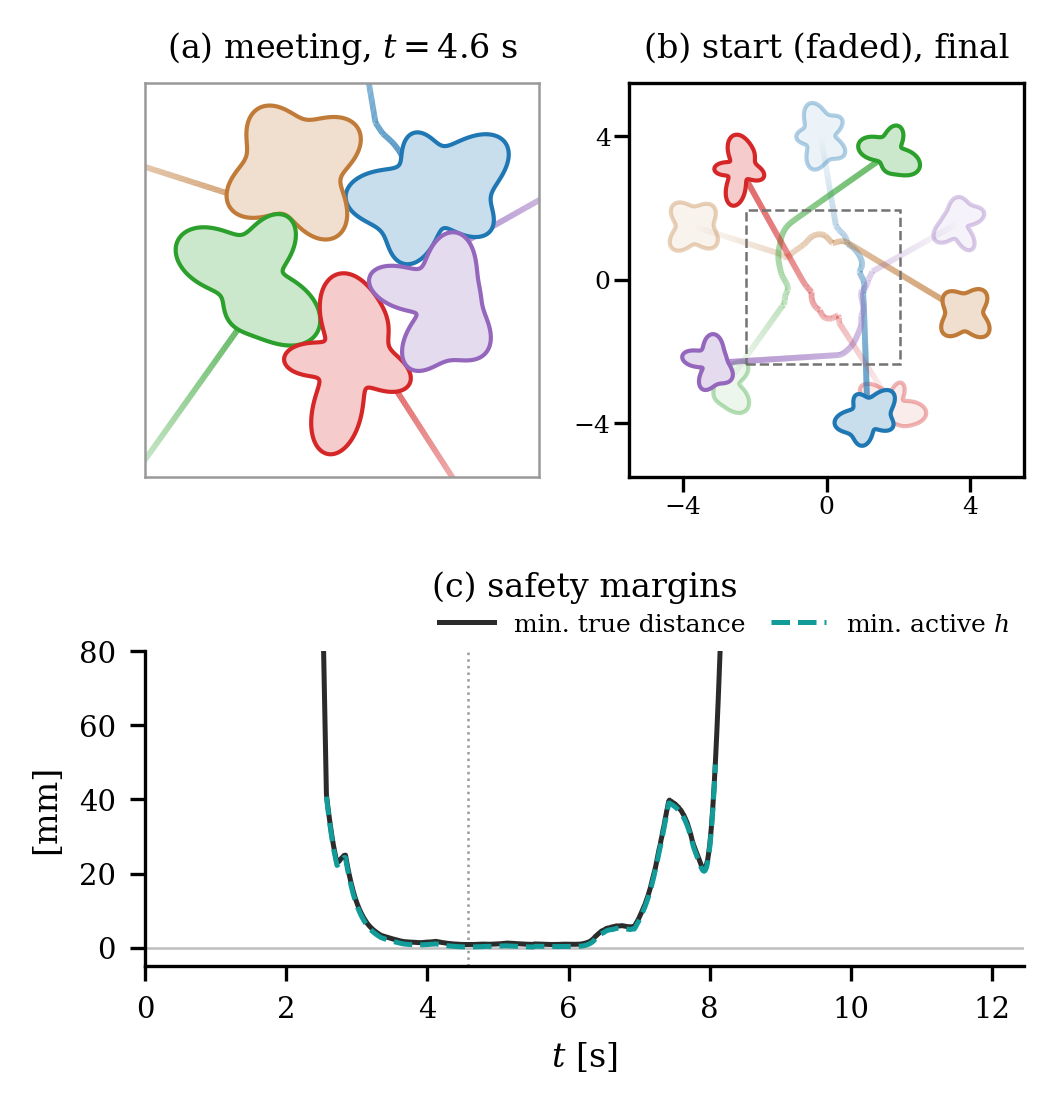
\includegraphics[width=0.92\columnwidth]{five_paper.png}
\caption{Five robots with random non-convex shapes exchanging positions under the surface-cover
barriers (pale fills: ground truth; darker outlines of the same hue: certified level curves).
(a) The five meet in the center at
$t=4.6$~s, when the most constraints are active (dashed square in (b)), with their paths so far.
(b) Start (faded) and final poses with center paths, drawn from faint (start) to strong (end).
(c) Minimum ground-truth distance over all pairs and certified lower bound of the lifted barriers
$\tilde h$ over the active boxes; dotted: the moment of (a).}
\label{fig:five}
\end{figure}

\begin{table}[t]
\caption{Twenty Random Five-Robot Instances}
\label{tab:stats}
\centering
\footnotesize
\setlength{\tabcolsep}{4pt}
\renewcommand{\arraystretch}{1.05}
\begin{tabular}{lccc}
\toprule
& ours & closest point & circle\\
\midrule
instances with a collision & \textbf{0} & 5 & \textbf{0}\\
min.\ evaluated distance [mm] & $+0.6$ & $-86.8$ & $+42.7$\\
min.\ $h$ [mm] & \textbf{0.0} & $-114.4$ & --\\
instances, all goals reached & 12 & 12 & \textbf{20}\\
constraints, max. & 1020 & 10 & 10\\
time/step, med./max.\ [ms] & 2.0/10.2 & 2.5/18.7 & 0.38/0.8\\
\bottomrule
\end{tabular}
\\[3pt]
\parbox{\columnwidth}{\footnotesize Horizon 15~s, step 10~ms. Negative distances: depth of the
deepest vertex inside the other polygon. Ours: $h$ is the certified lower bound of $\tilde h$ over the
active boxes. No step required slack. Time: median over instances of the per-instance median, and
maximum; one CPU thread.}
\end{table}

With the same shapes at half size, 20 random instances with poses in $[-3,3]^2\times\Sone$ compare
the barriers under single-integrator dynamics (Table~\ref{tab:stats}). The closest-point barrier
collides in 5 instances, with vertices up to 87~mm inside the other body: the closest pair of
non-convex bodies jumps, the derivative is one-sided, and the constraint normal can point the wrong
way just before contact. These results concern this single-closest-pair construction, the one
analyzed in~\cite{jo2026geometry}, not nonsmooth formulations over all active features. Ours and the
circles never collide; the circles reach all goals, whereas ours deadlocks in 8 instances, because
exact non-convex boundaries can hook where round surrogates slide past. On the 12 instances completed
by all methods, our mean path length is within 1\% of each baseline and our mean arrival time
within 10\%, ours being the
slowest because its remainders restrict the speed of bodies that slide close to each other: the
benefit of exact geometry appears in tight interactions such as docking. Ours lets the robots pass
within 0.6~mm, and the certified lower bounds of its lifted barriers stay nonnegative; it uses up to
255 active boxes (1020 constraints) at 2.0~ms per step (median; maximum 10.2~ms). The offline cost
for these half-size bodies is 14.5~s in total, about 3~s per body.

\subsection{Static Obstacles}\label{sec:exp-static}
A rocket-shaped robot (0.54~m long, nose, fuselage, two fins) escapes a curved maze (Fig.~\ref{fig:static}). The passage is our own design: three horizontal passes,
each with a smooth wiggle, joined by semicircular hairpins of radius 1.1~m, with a half-width of
0.43--0.51~m, entering and leaving the $8.9\times8.9$-m frame at right angles through straight
sections of equal length, 1.14~m. The two wall regions
are the frame minus this passage, combined through a smooth maximum of signed distances so that all
corners are rounded; their ground truth consists of cubic spans, sampled into polygons with a
certified chord deviation below 0.1~mm. One bivariate field with 1.25-cm cells ($791\times791$,
fitted in 40~s) encodes both walls, with a tightest level of 0.66~mm certified on the cubic spans in
0.5~s (Proposition~\ref{prop:level}, with the chord bound added to the piece radius), and the rocket's
field (1-cm cells, level 1.43~mm) is covered by 383 boxes of 5~mm. The nominal controller moves
toward eight waypoints using constant-speed pursuit with $v_{\max}=0.8$~m/s and
$\omega_{\max}=1.4$~rad/s. Their straight connections cut into the walls by up to 10~cm, so the barriers
keep the rocket off the walls: they modify the nominal input in 41\% of the 3242 steps while the
rocket slides along the walls to the exit in 32.4~s (path length 23.5~m), with up to 126 active boxes
(504 constraints). The ground-truth distance at the steps is at least 4.69~mm, and a conservative audit
that subtracts half of each step's motion verifies at least 0.59~mm between steps; the certified lower
bound of $\tilde h$ on the active boxes stays above 2.7~mm. The online cost is
1.9~ms per step (median; 95th percentile 3.7~ms), measured on one CPU thread with background
activity not excluded.

\begin{figure}[t]
\centering
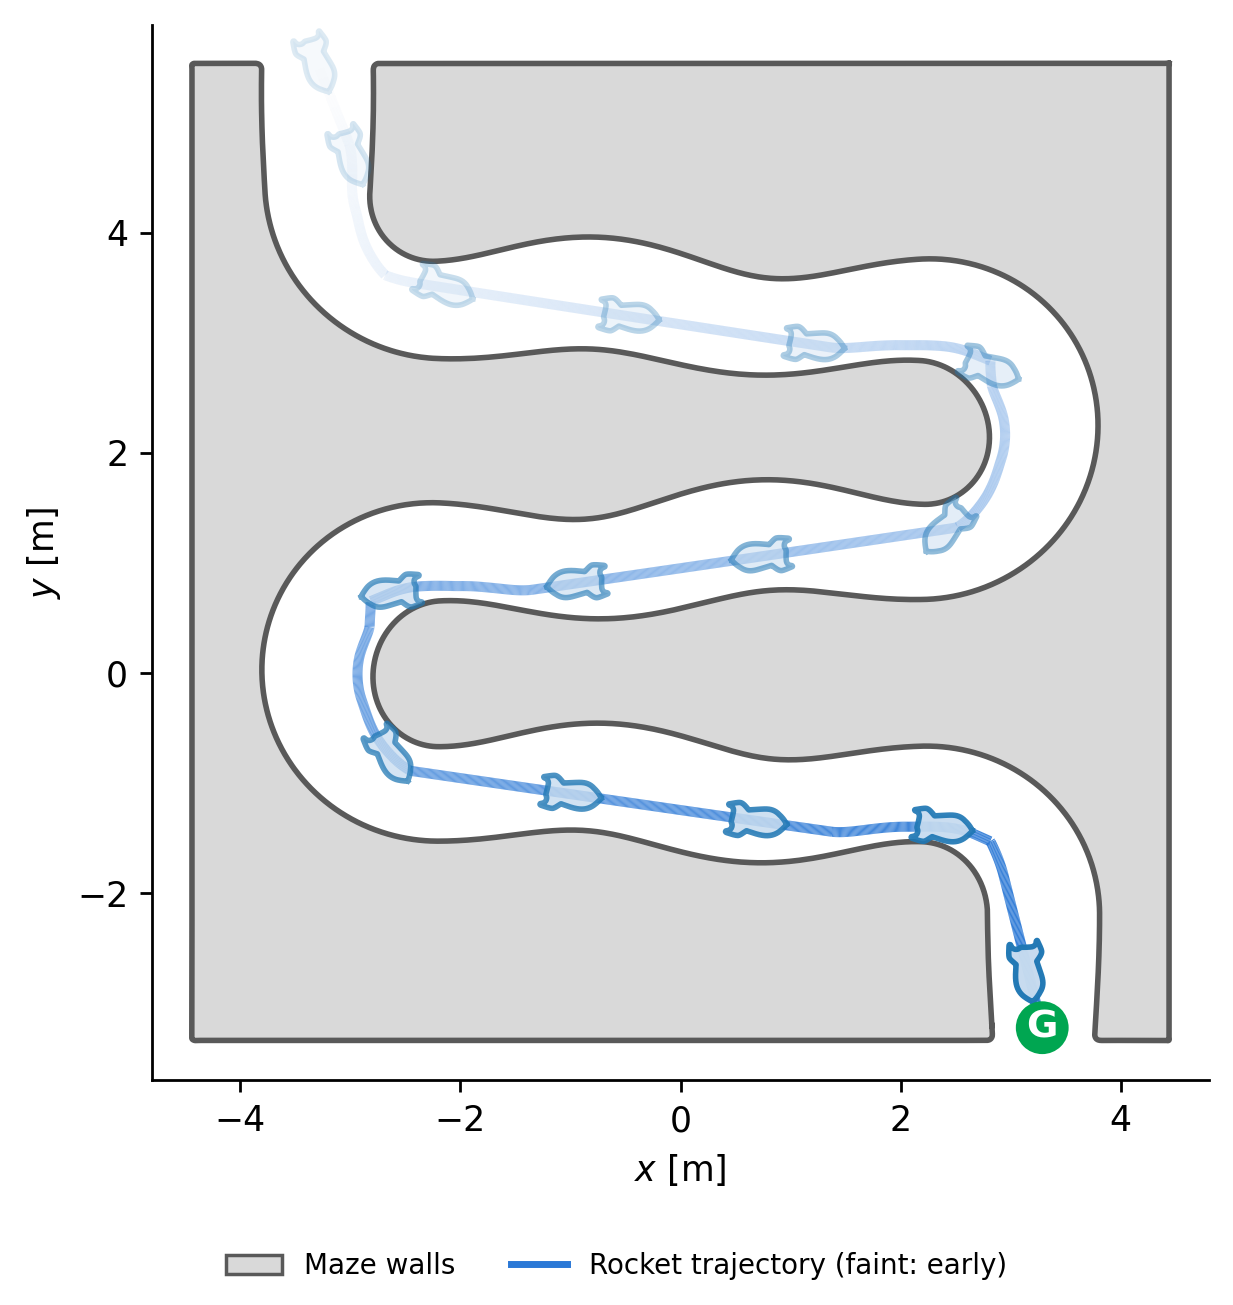
\includegraphics[width=0.8\columnwidth]{rocket_maze.png}
\caption{Escape of a rocket-shaped robot through a curved maze with surface-cover barriers and eight
goal waypoints, from the top entrance to the exit G. Gray fill with dark-gray outlines: walls (ground
truth and certified level curve); light-blue fill with blue outlines: the rocket at intermediate times
(ground truth and certified level curve); blue: path of its reference point. Poses and path are drawn from faint
(start) to strong (end).}
\label{fig:static}
\end{figure}

\subsection{Franka Panda among Non-Convex Obstacles}\label{sec:exp-franka}
The subdivided surface-cover barriers of Sec.~\ref{sec:cover} are applied to a 7-DOF Franka Panda with the link
meshes and kinematics of~\cite{li2024representing}. All eight links (the hand, without fingers, and
links 1--7) are constrained against three non-convex obstacles made of rounded boxes: a gate, an
inverted J, and a plate carrying a 2.4-cm rod on a leg, i.e., 24
link--obstacle pairs. Each link SDF is a cubic B-spline with 12-mm cells, fitted to approximate
signed distances of its mesh; its tightest level (1.8--3.8~mm) is certified on the mesh by
Proposition~\ref{prop:level} in 0.3--2~s, and its certified surface is covered by 1440--4420 boxes of
side 6~mm ($r=5.2$~mm). The obstacle fields have 2-cm cells, tightest levels of 1.9--2.9~mm, and
domains extending 15~cm beyond the obstacles. The joints are velocity-controlled ($|\dot q_j|\le1$~rad/s) with a proportional
joint-space nominal controller, $\gamma=5$, a 10-ms step, and activation threshold $\eta=3$~cm.

Start and goal configurations are drawn uniformly within 80\% of the joint ranges with the hand
above 0.1~m and a clearance of at least 3~cm, and we keep the first 30 pairs whose unfiltered motion
collides. At saved states, the link meshes are subdivided to edges below 4~mm
(same surface). The minimum of the obstacle's primitive SDFs is 1-Lipschitz and equals distance
outside their union; its value at each triangle centroid minus the triangle radius bounds it
over that entire triangle. A positive bound certifies separation. A negative bound alone does
not prove collision: we require a negative value at an actual mesh point and adaptively subdivide
triangles to resolve inconclusive bounds. All audited saved-state trials are resolved as having
a collision witness or positive separation bounds. As baselines, we use the 54
collision spheres of the Franka model in~\cite{li2024representing} and about 256 surface samples per
link, as in the collision-avoidance experiments of~\cite{li2024representing}, each with one barrier
per primitive and obstacle, the same primitive-SDF minimum, and a 1-cm margin.

\begin{figure*}[t]
\centering
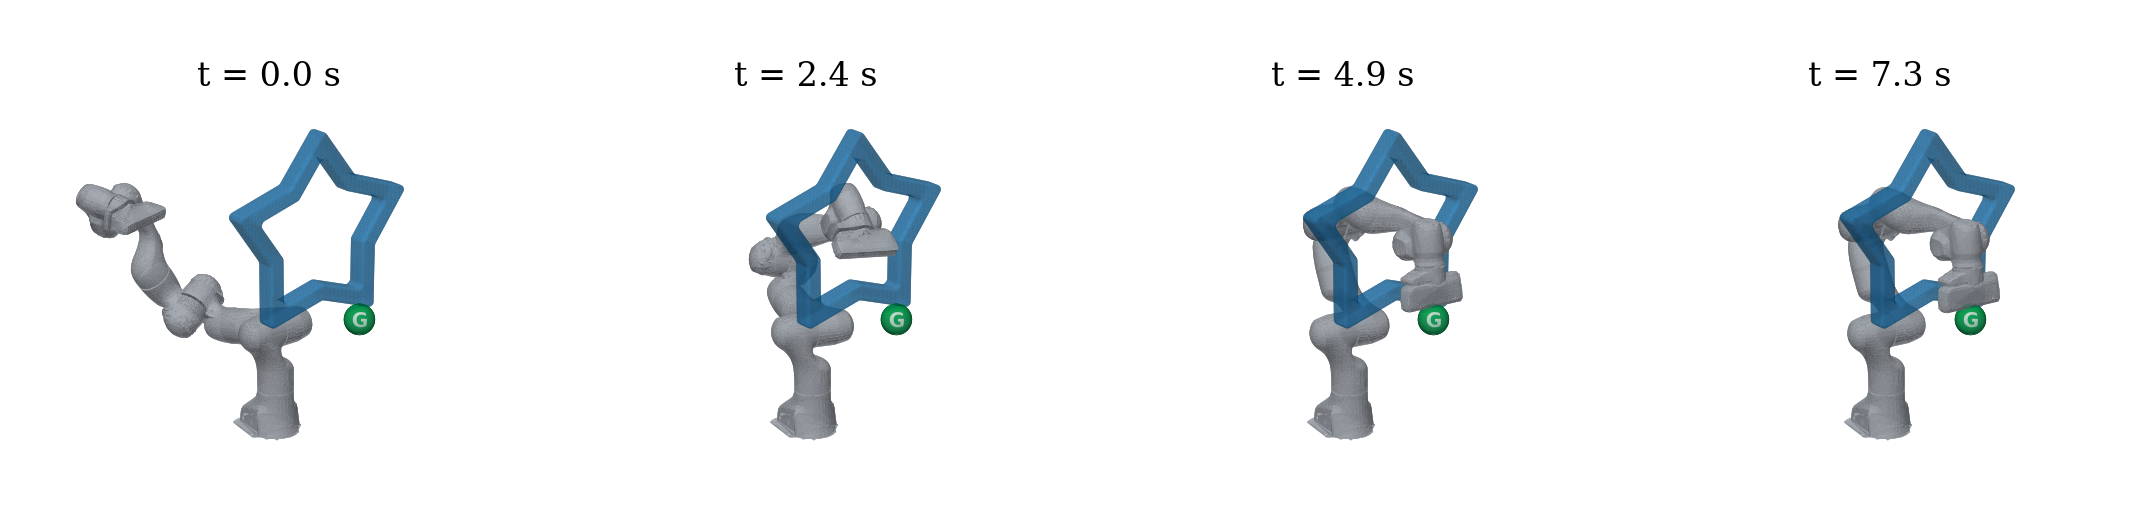
\includegraphics[width=\textwidth]{star_paper.png}
\caption{Franka Panda threading its forearm through a rounded star-shaped tube (blue; 5-pointed
star hole, nominal 5-cm walls, 6.7~cm deep) with the surface-cover barriers of all eight links.
The hand is within 1~cm of the goal G after 3.99~s; the last frame shows the settled pose.
Without the filter, the same nominal motion intersects the tube wall.}
\label{fig:star}
\end{figure*}

\begin{table}[t]
\caption{Franka Panda: 30 Trials Whose Unfiltered Motion Collides}
\label{tab:franka}
\centering
\footnotesize
\setlength{\tabcolsep}{2pt}
\renewcommand{\arraystretch}{1.05}
\begin{tabular}{lcccc}
\toprule
& ours & spheres & samples & KKT\\
\midrule
primitives & 26{,}636 & 54 & 1975 & 24\\
surface certificate & yes & no & no & no\\
trials with collision witness & \textbf{0} & 0 & 0 & 5\\
\quad without margin & -- & 13 & 15 & --\\
\quad min. field bound [mm] & -- & $-10.2$ & $-13.4$ & $-41.9$\\
saved-state min. [mm] & 1.1 & 0.9 & 1.4 & $<0$\\
median of the minima [mm] & 5.7 & 8.6 & 7.2 & 2.4\\
trials reaching the goal & 17 & 20 & 23 & 20\\
trials needing slack & 0 & 0 & 0 & 7\\
time/step, med./p95 [ms] & \timeOurs & \timeSph & \timePts & \timeKKT\\
constraints, max. & 34{,}992 & 21 & 188 & 5\\
\bottomrule
\end{tabular}
\\[3pt]
\parbox{\columnwidth}{\footnotesize Without the filter, all 30 trials collide. Primitives: initial cover boxes
(optional online halving adds children),
spheres, surface samples, and closest-point pairs. Spheres and samples: primitive-SDF minimum with a
1-cm margin unless stated; KKT: the certified fields and levels of ours. Distances: certified lower
bounds between the link meshes and the obstacles at saved states; they do not bound between-step motion.
Every trial without a collision witness has positive separation bounds at its evaluated states.
Minimum field bounds use the margin-free sphere/sample runs and KKT. Negative values bound
the minimum-of-primitives defining field and are not penetration depths.
The continuous-surface certificate assumes exact arithmetic and feasible continuous-time enforcement.
Time per step: median and 95th percentile over all steps of the 30 trials, one CPU thread
(Python, AMD Ryzen~9 3900X).}
\end{table}

In all 30 trials, our filtered arm has positive saved-state mesh-distance lower bounds
(Table~\ref{tab:franka}), with a minimum of 1.1~mm between meshes and obstacles
(median over trials 5.7~mm); no step
requires slack, and the certified lower bounds of the lifted barriers stay nonnegative. Each certified
level is a bound on field values at the mesh surface, not a physical offset distance. The local
fitting error therefore allows the meshes to come closer than the sum of the two levels
(at least 3.7~mm). Barriers at the box corners that
bound $\phi_O$ alone kept 8.4~mm in the same trials. Within the 10-s horizon, the arm reaches the goal in 17 trials, against
23 with those corner barriers: close to an obstacle, the remainders of~\eqref{eq:coef} slow the links
that slide along it, and in the other trials the arm stops in front of an obstacle. The filter needs
\timeFrankaMed~ms per step (median; 95th percentile \timeFrankaPninetyfive~ms) with up to 4374 active
boxes (34{,}992 constraints). Both timing statistics exceed the 10-ms simulation step, so these
runs do not establish a 100-Hz real-time implementation.
Restricting to the 70\% of steps with at least one active box gives median/p95 times of
17.3/57.5~ms; the maximum over all steps is 237.6~ms.

With a 1-cm margin, both baselines have positive saved-state mesh-distance lower bounds
(minima 0.9 and 1.4~mm): the margin, not a certificate, absorbs the geometric error of the
primitives. Without the margin, collision witnesses occur in 13 sphere trials and 15 surface-sample
trials. Their minimum defining-field lower bounds are $-10.2$ and $-13.4$~mm, respectively;
these values are not penetration depths. The spheres do not enclose the meshes, and the samples
leave parts of the surface unconstrained,
although every sampled barrier stays above $-0.05$~mm: the obstacle enters between the samples. The baselines are
cheaper per step and reach the goal more often (20 and 23 trials); what the surface cover adds is
that the constraint holds on the whole continuous surface, so that no margin has to be tuned.
Finally, the closest-point barrier of~\cite{jo2026geometry}, transferred to 3D with the same
certified fields and levels (one barrier per link--obstacle pair at
$\mathbf x^\ast=\argmin\phi_O$ subject to $\phi_A=l_A$, SLSQP warm-started from the previous step),
has collision witnesses in 5 trials, a minimum defining-field lower bound of $-41.9$~mm,
violates its own barrier by up to 37~mm, needs slack in 7, and costs 128~ms per step:
this warm-started local solver does not ensure a global minimum or smooth tracking between
surface patches on non-convex links.

\emph{Threading a rounded star-shaped tube.} Fig.~\ref{fig:star} shows a tighter static scene,
arranged in an interactive tool and replayed. A 6.7-cm-deep tube with a 5-pointed star hole and
nominal 5-cm walls stands 0.65~m high in front of the arm. The cross-section is constructed from
stars with hole-tip and notch radii of 24 and 15~cm; the corners are filleted with radius 15~mm,
and the front and rear edges with radius 10~mm. This rounded solid is the ground truth, with an
analytic distance function; its fitted field has 1.5-cm cells and a certified level of 1.6~mm.
The arm starts beside the tube and a damped-least-squares IK moves the hand to the home pose,
which puts the forearm through the hole. The unfiltered motion intersects the wall.
With the filter, the hand reaches the 1-cm goal tolerance after 3.99~s of simulated time.
Over the 15-s run, all 1501 saved states have a mesh-distance lower bound of at least 1.00~mm
(the audit's bound-reuse threshold),
and no step needs slack. This audit covers every modeled link triangle using 4-mm subdivisions,
the analytic distance function, and geometric bounding-box pruning. A previous link bound can
be transferred to a new pose by subtracting
$\norm{\mathbf t-\mathbf t_0}+\norm{\Rot-\Rot_0}r_L$, where $r_L$ bounds the norm of every
point in the link's frame; otherwise its triangles are evaluated again. It uses no fitted-field
cutoff and does not certify the motion between saved states.
Rounding alone does not remove the stall: with refinement restricted
to boxes whose lifted lower bound is below 1~cm, the arm still fails to reach within 15~s.
Allowing every active box whose remainder exceeds $\vartheta$ to be refined yields the successful
run, with up to 3961 boxes (31{,}688 constraints) and 77/103~ms median/95th-percentile filter time.
These computation times exceed the 10-ms simulation step; this experiment does not demonstrate
a 100-Hz real-time implementation.

\subsection{Two Franka Pandas in a Shared Workspace}\label{sec:exp-dual}
\begin{figure*}[t]
\centering
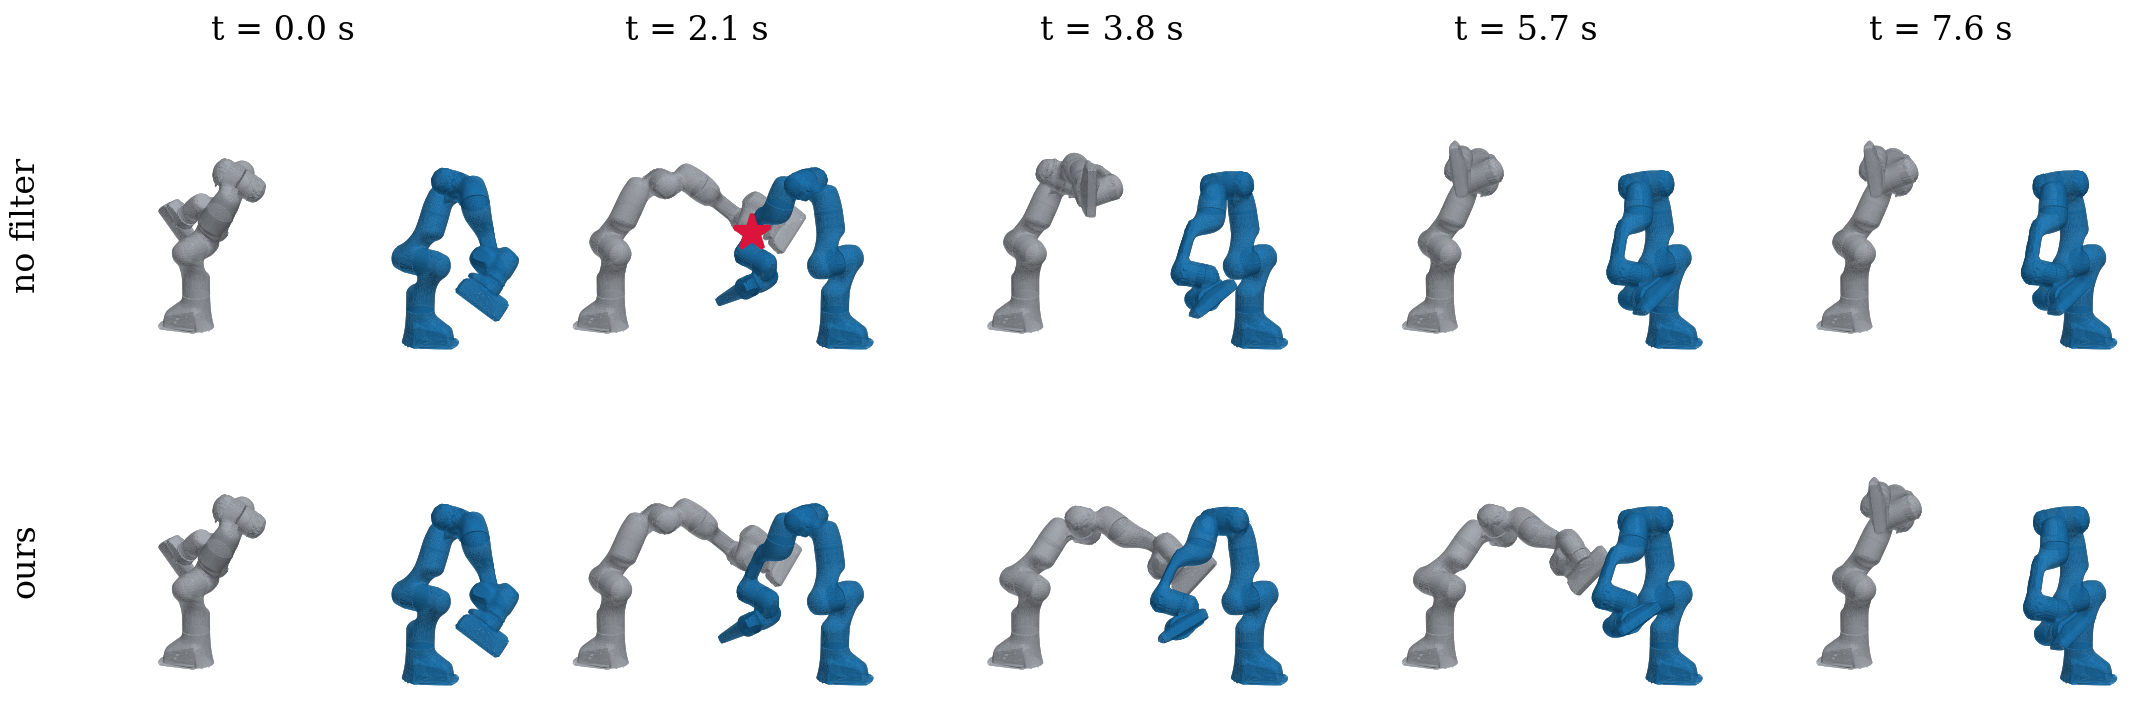
\includegraphics[width=\textwidth]{dual_paper.png}
\caption{Two Franka Pandas move to their goals and cross. Top: unfiltered motion; red stars mark
sampled mesh pairs less than 2~mm apart. Bottom: with the surface-cover barriers of
all 64 link pairs, arm~1 (gray) and arm~2 (blue) slide past each other and both reach their goals,
7.6~s after the start.}
\label{fig:dual}
\end{figure*}
Two Franka Pandas face each other with bases 0.9~m apart. For each of the 64 pairs of a link of arm~1
and a link of arm~2, the certified surface of the first is bounded against the SDF of the second;
both links move, so each constraint is affine in the velocities of all 14 joints (the
derivative in Sec.~\ref{sec:cover} with the Jacobians of both arms), and one direction per pair
suffices by Theorem~\ref{thm:cover}. Starts and goals of both arms are drawn as before, with an
initial clearance of 5~cm, and we keep the first 20 of 143 sampled pairs whose unfiltered motion
reduces the sampled mesh distance below 2~mm. This proximity threshold selects challenging
trials; it does not by itself establish intersection. The distance between the arms is
bounded from below with exact point-to-triangle distances from the subdivided triangles of arm~1 to
the meshes of arm~2, at up to 20 steps per trial whose sampled distances lie within 5~mm of the
sampled minimum. A mesh-to-sample cover bound of at most 6.84~mm validates sample-based pruning;
all omitted terms retain a 20-mm lower bound. All these
audited states have positive lower bounds and all 20 trials use zero slack
(Fig.~\ref{fig:dual} shows one); the barriers are active
($\min h<5$~mm) in 8 trials, the
sampled mesh distances fall below 3~cm in 16, and the minimum certified lower bound over the
audited states is 1.6~mm, below the
sum of the two levels of a pair of links for the same reason (corner barriers on $\phi_B$ alone kept
10.3~mm). Both arms reach their
goals in 15 trials (17 with the corner barriers). The filter needs \timeDualMed~ms per step (median;
95th percentile \timeDualPninetyfive~ms) with up to 6730 active boxes (53{,}840 constraints) over the
64 link pairs. Over the 48\% of steps with at least one active box, median/p95 time is
31.2/104.6~ms; the maximum over all steps is 447.5~ms.
For broad-phase pruning, spheres of radii $R_A,R_B$ enclose all cover boxes. Pairs with
$\norm{\mathbf p_A-\mathbf p_B}>R_A+R_B+0.06\,\mathrm m+\eta$ are omitted; Bernstein bounds
on every field cell intersecting $\{\norm{\mathbf y}\ge R_B+0.06\,\mathrm m+\eta\}$ certify
$\phi_B-l_B\ge86.5$~mm there. The domain-collar certificate handles points outside the field.
This selected-state audit does not certify the minimum over all saved states or
between them.

% -----------------------------------------------------------------------------
\subsection{Comparison of Finite Certificates}\label{sec:cert-comparison}
We compare the vertex reduction (V) and the joint Bernstein certificate (B) while keeping
the spline fields, certified levels, and initial covers identical. All variants use
distance-independent refinement with $\vartheta=0.1$ and at most two halvings; screening
uses the unit lift. In addition to $w=1$, we test fixed multipliers with
$\mathbf a=\nabla\phi_A(\mathbf c)$, $\mathbf b=\Rot^\top\nabla\phi_B(\mathbf y_{\mathbf c})$,
\begin{equation}
w_{\rm N}=\sqrt{\frac{\norm{\mathbf b}^2+\delta}{\norm{\mathbf a}^2+\delta}},\qquad
w_{\rm P}=-\frac{\mathbf a^\top\mathbf b}{\norm{\mathbf a}^2+\delta},\quad\delta=10^{-12}.
\end{equation}
The regularizer keeps the weights continuous at zero gradient. Negative projection weights
are permitted, with the absolute value in the remainder of~\eqref{eq:joint-model}.
Neither choice cancels the complete, input-dependent spatial gradient of the CBF condition.

Table~\ref{tab:cert-comparison} uses fixed horizons of 9~s for docking and 6~s for the rounded
tube. The input modification is $J=\int\norm{\mathbf u-\mathbf u^{\rm nom}}\,dt$, compared
only within each scene. All twelve runs require zero slack. Docking has positive polygon-distance
bounds; the independent tube audit covers all 601 saved states per variant and every modeled mesh
triangle, using the analytic obstacle field and a 1-mm bound-reuse threshold, without fitted-field
pruning. All six tube lower bounds remain above 1~mm. The docking runs seat the vehicle; the nominal target is intentionally
10~cm beyond full seating, so reaching that infeasible target is not the docking success criterion.

\begin{table}[t]
\caption{Certificate Comparison with Fixed Geometry}
\label{tab:cert-comparison}
\centering\footnotesize
\setlength{\tabcolsep}{3pt}
\begin{tabular}{lrrrr}
\toprule
Certificate & Dock $J$ & Tube $t_g$ [s] & Tube $J$ & Tube time [ms]\\
\midrule
V, $w=1$       & 0.656 & 3.99 & 1.948 & 34.6/83.7\\
B, $w=1$       & 0.653 & 3.93 & 1.870 & 52.2/165.7\\
V, $w_{\rm N}$ & 0.655 & 3.99 & 1.951 & 33.9/85.3\\
B, $w_{\rm N}$ & 0.653 & 3.92 & 1.857 & 52.2/165.6\\
V, $w_{\rm P}$ & 0.655 & 4.00 & 1.965 & 34.7/83.3\\
B, $w_{\rm P}$ & 0.653 & 3.95 & 1.896 & 51.0/166.5\\
\bottomrule
\end{tabular}
\\[3pt]
\parbox{\columnwidth}{\footnotesize $t_g$: simulated goal-arrival time. Filter time: median/p95
over the fixed 6-s horizon, one CPU thread. These are exploratory measurements with background
activity not excluded, rather than the isolated timings of Table~\ref{tab:franka}. The tube's
15-s experiment above has a different timing distribution.}
\end{table}

The joint unit-weight certificate reduces tube input modification by about 4\%, at the cost
of increasing the maximum row count from 26{,}440 to 89{,}424. The fixed multipliers do not
improve the vertex variant's tube arrival time or input modification. These cases therefore
support retaining the unit-weight vertex reduction as the economical implementation, while
the joint coefficient condition provides a direct alternative when the additional cost is
acceptable. The multiplier tests establish neither a general improvement nor a second-order
conservatism result.

We also compare the two unit-weight certificates on six saved Franka trials, selected as three
that reached and three that stalled in the original experiment. With the same distance-independent
refinement, both variants reach in four of six trials and require zero slack in all six.
For the newly successful trial, the joint certificate reduces arrival time from 7.38 to 6.63~s
and $J$ from 4.243 to 3.533; its median/p95 filter time increases from 46/116 to 73/250~ms.
In the most expensive trial neither variant reaches within 10~s, while median filter time rises
from 115 to 253~ms and maximum row count from 41{,}776 to 146{,}691. These selected trials
show a cost--performance tradeoff, not a new estimate of the 30-trial success rate.

\section{Limitations}\label{sec:limits}
\emph{Certificates.} The certificates exclude first contacts, so they protect trajectories that
start collision-free, and they certify non-intersection, not a prescribed clearance (which follows
by enclosing dilated ground truths). They assume exact arithmetic; our implementation uses double
precision without outward rounding.

\emph{Closed-loop solutions.} The corollary is conditional on an absolutely continuous solution
with feasible controls satisfying the certificates almost everywhere. It does not establish
existence or uniqueness for the QP feedback with hard activation and optional refinement, or
admissibility of every Filippov selection. A positive activation threshold alone does not make
entering constraints redundant. Enforcing rows only at simulation steps does not meet the
almost-everywhere hypothesis between those steps.

\emph{Discrete time.} The guarantees hold in continuous time. The simulations use 10-ms steps;
distance checks at saved states do not certify the motion between them. Sampled-data CBF
conditions account for the held input and intersample evolution~\cite{breeden2022sampled};
adapting such a tightening is needed for a guarantee of the implemented controller.

\emph{Conservatism, feasibility, and cost.} The safe set is defined by the continuous spline level
surfaces. Its finite enforcement is conservative: Taylor remainders and Bernstein bounds restrict
the admissible inputs. Proposition~\ref{prop:tight} bounds the constant-term loss, which is first
order in box size where the two field gradients do not cancel; it does not give a general physical
clearance penalty. The constraints can slow motion where the fields vary quickly and certify
stopping only when their constant terms are nonnegative. Finer boxes reduce these losses at the
price of more constraints. Their number,
$2^n$ per active box and thousands in tight spatial scenes, sets the cost per step and its
variation.

\emph{Online geometry.} The robot's fields, levels, and covers are prepared once; a new obstacle needs
only its own field and certified level, which took 0.1--0.2~s and 2--13~s, respectively, for the
Franka obstacles in our Python implementation: enough for occasional updates, not for every sensor
frame. For perceived obstacles, the certificate holds for the reconstructed geometry.

\emph{Scope.} Deadlocks are not resolved, and exact geometry makes them more frequent than round
surrogates. The manipulator studies omit self-collision within an arm, the fingers, and polytopic
baselines, and all experiments are in simulation.

% -----------------------------------------------------------------------------
\section{Conclusion}\label{sec:concl}
Collision avoidance between non-convex rigid bodies reduces, through a first-contact lemma, to
keeping each body's SDF above a certified level on the boundary of the other. We took this condition
on the continuous level set as the safe set and enforced it through Bernstein bounds of a lifted
barrier on a cover of that level set, so that the finite certificate restricts only the inputs, for
planar and spatial, rigid and articulated bodies, with one field per body. Native SDF patches form
the default cover, without an independent cover resolution or online refinement. The construction computes
no closest points and certifies the required strict inclusion of the true boundaries. With optional subdivision, it never collided in planar
experiments, unlike a closest-point barrier, docked where bounding circles cannot, kept a Franka
Panda's saved-state mesh-distance bounds positive within millimeters, and produced positive
distance bounds at the audited two-Panda states. Sampled-data
guarantees, faster enforcement near contact, deadlock resolution, and hardware validation are the
next steps.

\bibliographystyle{IEEEtran}
\bibliography{references}

\end{document}
